%% Version: 0.8 (12.02.2019)

%% thesis.tex
%% Copyright 2020 KIT, IAR-IPR (Denis Štogl)
%% Mail: denis.stogl@kit.edu
%
% This work may be distributed and/or modified under the
% conditions of the LaTeX Project Public License, either version 1.3
% of this license or (at your option) any later version.
% The latest version of this license is in
%   http://www.latex-project.org/lppl.txt
% and version 1.3 or later is part of all distributions of LaTeX
% version 2005/12/01 or later.
%
% This work has the LPPL maintenance status `maintained'.
%
% The Current Maintainer of this work is M. Y. Name.
%
% This work consists of the files pig.dtx and pig.ins
% and the derived file thesis.tex.

%% Choose language: english or german
%% Choose Thesis type: seminar, bachelor, master, phd, techreport
%% Use 'declaration' parameter if you want to generate declaration page
%% Use 'final' to disable Todo-notes from final version without deleting each one of them
\documentclass[english,master]{KITthesis}

%% ---------------------------------
%% | Information about the thesis  |
%% ---------------------------------
%% Version: 0.8 (12.02.2019)

%% My_document_info.tex
%% Copyright 2020 KIT, IAR-IPR (Denis Štogl)
%% Mail: denis.stogl@kit.edu
%
% This work may be distributed and/or modified under the
% conditions of the LaTeX Project Public License, either version 1.3
% of this license or (at your option) any later version.
% The latest version of this license is in
%   http://www.latex-project.org/lppl.txt
% and version 1.3 or later is part of all distributions of LaTeX
% version 2005/12/01 or later.
%
% This work has the LPPL maintenance status `maintained'.
%
% The Current Maintainer of this work is M. Y. Name.
%
% This work consists of the files pig.dtx and pig.ins
% and the derived file thesis.tex.


\title{Distributed Control of Multiple Robots Using ros2\_control}

\titleotherlanguage{Verteilte Mehrmaschinen-Regelung einer Roboterzelle mittels ros2\_control
}

\author{Manuel Muth}
\address{Berckmüllerstraße 1C}
\city{76131 Karlsruhe}
\email{uqdut@student.kit.edu}

\keywords{distributed control, multiple controllers, ros2\_control, ROS2, control}
\keywordsotherlanguge{verteilte Regelung, mehrere Regler, ros2\_control, ROS2, Regelung, Regelungstechnik}

%% Study program or a seminar/subject
\studyprogram{Intelligente Industrieroboter}

%% IMPORTANT: Seminar only: If not "Seminar Intelligente Industrieroboter" uncomment this
% \nogrouplogo

%% Name of your institute (Default: IAR-IPR)
% \institute{Test}
%% Name of your faculty (Default: KIT-Fakultät für Informatik
% \KITfaculty{This is my Faculty}
%% Address of your institute (Default: Engler-Bunte-Ring 8)
% \instituteaddress{}
% %% Insitute City (Default: 76131 Karlsruhe)
% \institutecity{}

\reviewerone{Prof. Dr.-Ing. habil. Björn Hein}
\reviewertwo{Prof. Dr.-Ing. habil. Thomas Längle}
%
% %% The advisors are PhDs or Postdocs
\advisorone{Dr.-Ing. Denis \v{S}togl}
% %% The second advisor can be omitted
\advisortwo{}
%
% %% Please enter the start end end time of your thesis (for techreport not needed)
\editingtime{03. Januar 2023}{03. Juli 2023}

%% --------------------------------
%% | Settings for word separation |
%% --------------------------------
% Help for separation:
% In german package the following hints are additionally available:
% "- = Additional separation
% "| = Suppress ligation and possible separation (e.g. Schaf"|fell)
% "~ = Hyphenation without separation (e.g. bergauf und "~ab)
% "= = Hyphenation with separation before and after
% "" = Separation without a hyphenation (e.g. und/""oder)

% Describe separation hints here:
\hyphenation{
% Pro-to-koll-in-stan-zen
% Ma-na-ge-ment  Netz-werk-ele-men-ten
% Netz-werk Netz-werk-re-ser-vie-rung
% Netz-werk-adap-ter Fein-ju-stier-ung
% Da-ten-strom-spe-zi-fi-ka-tion Pa-ket-rumpf
% Kon-troll-in-stanz
}

%%
%% --------------------
%% |   Bibliography   |
%% --------------------
\newcommand{\mybibliographyfiles}{Bibliography/ipr_articles,Bibliography/kit_template_example_bibliography,Bibliography/masterthesis}


%% --------------------
%% |     Acronyms     |
%% --------------------
\newacronym{dof}{DOF}{Degree of Freedom}
\newacronym{dds}{DDS}{OMG Data-Distribution Service}
\newacronym{ipr}{IAR-IPR}{Institute for Anthropomatics and Robotics - Intelligent Process Control and Robotics}
\newacronym{kit}{KIT}{Karlsruhe Institute of Technology}
\newacronym{qos}{QoS}{Quality of Service}
\newacronym{ptp}{PTP}{Precision Time Protocol}
\newacronym{rcl}{rcl}{\gls{ros} Client Library}
\newacronym{rclcpp}{rclcpp}{\gls{ros} Client Library C++}
\newacronym{rclpy}{rclpy}{\gls{ros} Client Library Python}
\newacronym{rmw}{rmw}{\gls{ros} middleware}
\newacronym{ros}{ROS}{Robot Operating System}
\newacronym{ros2}{ROS 2}{Robot Operating System 2}
\newacronym{rsi}{RSI}{RobotSensorInterface}
%% --------------------
%% |     Glossary     |
%% --------------------
\newglossaryentry{ci}
{
    name={\textit{CommandInterface}},
    description={}
}
\newglossaryentry{ddsg}
{
    name={\gls{dds}},
    description={\acrlong{dds} publish-subscribe a communication based middleware standard for real-time and embedded systems by \cite{pardo-castellote_omg_2003, schlesselman_omg_2004, noauthor_data_nodate}}
}
\newglossaryentry{dofg}
{
    name={\gls{dof}},
    description={\acrlong{dof}}
}
\newglossaryentry{node}
{
    name={\textit{node}},
    description={Can be understood as a fundamental software component that is used for communication and computation in \gls{ros} and \gls{ros2}. Builds the organizing endpoint int the computional graph. It can perform various tasks such as sensing, actuating, processing, and interfacing with other nodes to exchange data or trigger actions},
    plural={\textit{nodes}}
}
\newglossaryentry{nodelet}
{
    name={\textit{nodelet}},
    description={Simliar to a \gls{node} in \gls{ros} but with the ability to run multiple nodlets in one process},
    plural={\textit{nodelets}}
}
\newglossaryentry{message}
{
    name={\textit{message}},
    description={Datatype in \gls{ros} and \gls{ros2} used when communication via \glspl{topic}},
    plural={\textit{messages}}
}
\newglossaryentry{rc}
{
    name={\textit{ros\_control}},
    description={Framework for robot control in \gls{ros}}
}
\newglossaryentry{ri}
{
    name={\textit{ReferenceInterface}},
    description={}
}
\newglossaryentry{rosg}
{
    name={\gls{ros}},
    description={The \acrlong{ros} is a middleware based on a publisher-subsciber model. \gls{rosg} is mainly used in robotics and provides services for hardware abstraction and low-level control. Further, it comprises tools, libraries, and functionalities used in robotic applications}
}
\newglossaryentry{ros2g}
{
    name={\gls{ros2}},
    description={\acrlong{ros2} is the second generation of the \acrlong{ros} \cite{macenski_robot_2022}}
}
\newglossaryentry{r2c}
{
    name={\textit{ros2\_control}},
    description={Framework for real-time capable control using \gls{ros2}}
}
\newglossaryentry{rsig}
{
    name={\gls{rsi}},
    description={The \acrlong{rsi} serves as an interface for communication between the industrial robot and its sensor system }
}
\newglossaryentry{service}
{
    name={\textit{service}},
    description={A service is a communication mechanism in \gls{ros} and \gls{ros2} that allows \glspl{node} to request and receive a response in a client-server pattern},
    plural={\textit{services}}
}
\newglossaryentry{si}
{
    name={\textit{StateInterface}},
    description={}
}
\newglossaryentry{sm}
{
    name={shared-memory},
    description={Shared-memory architecture is a concept that allows multiple processors or threads to access a common physical memory. Data can then be exchanged over the common memory. }
}
\newglossaryentry{topic}
{
    name={\textit{topic}},
    description={In the context of \gls{ros} and \gls{ros2} a topic is a communication mechanism. Topics provide a publisher-subscriber based exchange mechanism of \glspl{message} for \glspl{node}},
    plural={\textit{topics}}
}

%% ------------------------
%% |    Including files   |
%% ------------------------
% Only files listed here will be included!
% Userful command for partially translating the document (for bug-fixing e.g.)
% \includeonly{%
% Content/0-Declaration,
% Content/0-Abstract_EN,
% Content/0-Abstract_DE,
% Content/1-Introduction,
% Content/2-State-of-the-art,
% Content/3-Methods,
% Content/4-Concept,
% Content/5-Implementation,
% Content/6-Results,
% Content/7-Discussion,
% Content/8-Conclusion,
% Content/11-Appendix,
% }

\settitle
%%%%%%%%%%%%%%%%%%%%%%%%%%%%%%%%%
%% Here, main documents begins %%
%%%%%%%%%%%%%%%%%%%%%%%%%%%%%%%%%
\begin{document}
%% Uncomment this to use only first authors name in bibliography
% \bstctlcite{BSTcontrol}

%% Set PDF metadata
\setpdf

%% Title Page
\includetitle

% TODO: Remove this from final version
\includelistoftodos

\includedeclaration

\includeacknowledgments

%% ----------------
%% |   Abstract   |
%% ----------------
%% An abstract both in English
%% and German is mandatory.
%%
%% The text is included from the following files:
%% - Content/0-Abstract_EN
%% - Content/0-Abstract_DE
\includeabstract

%% ------------------------
%% |   Table of Contents  |
%% ------------------------
\inculdetableofcontents

\makenomenclature

%% -----------------
%% |   Main part   |
%% -----------------
\setmainpart

%% ==============================
% Part is used only in PhD thesis
\part{The challenges}
\chapter{\iflanguage{ngerman}{Einleitung}{Introduction}}
\label{sec:Introduction}
%% ==============================
\section{Motivation}\todo{check this again some useful additions to motivation:\cite{bilancia_overview_2023}}
Robots are playing a more and more vital role in every sector of our lives. This can be seen especially in the industrial, automotive and electronic field, where they have been increasingly used in the last 30 years \cite{cheng_rise_2019, bilancia_overview_2023}. However, robotic systems are also increasingly appearing in our everyday lives, whether through robotic vacuum cleaners or robotic mowers. The basis of all these robotic systems are the drivers and controllers that enable the control and thus the movement of these robotic systems. However, today many of the controllers for robotic control are monolithic black-boxes built by the robot manufacturers. Those black-boxes are neither accessible nor exchangeable. This is often due to the fact of them finely tuned to fulfill the task of robot control for the robots distributed by the manufacture \cite{puck_distributed_2020, plasberg_towards_2022}. \newline
With the appearance of \gls{ros} in 2007, an open-source framework for robotics development, and packages such as \gls{rc}, it is possible to combine those monolithic controllers with simply interfaces. This allows the creation of complex robotic applications. By 2009 \gls{ros} had established itself as 'de facto' standard for robotics software development. However, \gls{ros} has its limitations which lead to the development of second version. The second version, called \gls{ros2}, was built from the ground up with the goal of addressing those limitations. \newline
With \gls{ros2} the \gls{r2c} framework for real-time capable control emerged. The \gls{r2c} framework is a rewrite of \gls{rc} with the goal to simplify integration of new hardware and overcome drawbacks present in \gls{rc}. However, the current version of \gls{r2c} is focused on controlling a single robot or small robot cell and is based on a \gls{sm} architecture. This does not make use of the utilized middleware \gls{dds} with its full support for message exchange over the network. \newline

\section{Scope of this Thesis}
This thesis concentrates solely on \gls{ros2} and especially on the question of the feasibility to realize a distributed control concept over the network in \gls{r2c}. It aims to evaluate how such a concept could be integrated into the existing \gls{r2c} framework. Further, the goal is to test if the proposed concept is capable of controlling multiple robots. Moreover, is aims at evaluating what influence the chosen middleware of \gls{ros2} has. Respectively, chosen parameters and quality of service settings of the \gls{rmw} are compared and evaluated.


\section{Thesis Outline}
\paragraph{\hyperref[sec:state_of_the_art]{Section 2: State of the Art}}
The second chapter of this thesis provides an overview of recent work on the topic of controlling multiple robots in a distributed manner. Some papers which conducted studies on the real-time capabilities of \gls{ros2} and how this translates to the possibility of distributed control inside \gls{ros2} are presented.

\paragraph{\hyperref[sec:background]{Section 3: Background}}
In the third chapter, an overview and introduction to frameworks and technologies this thesis relies on is given. First, \gls{ros} as well as its successor \gls{ros2} are introduced. Then a quick introduction to the \acrlong{dds} is given and a quick overview of different middlewares for \gls{ros2} are presented. Thereafter, the current state of the \gls{r2c} framework is presented and the most important concepts for this thesis are introduced, like hardware abstraction and chaining of controllers. Further, it is shown how in the current version of \gls{r2c}, based on \acrlong{sm}, multiple robots can be controlled and what the drawbacks and limitations are.

\paragraph{\hyperref[sec:concept]{Section 4: Concept}}
In the fourth chapter, the concept that underlies this work is outlined. Different criteria the design should fulfill are presented, as well as control architectures that should be realizable with the approach. It is presented how this thesis is build on top of concepts from \gls{ros2} like \glspl{topic} and \glspl{service}. The overall design of the system with one central and multiple sub-controller managers is explained. The necessary steps for establishing a connection between central and sub-controller manager are explained. Further, the idea of how to integrate everything in the existing framework of \gls{r2c} without having to change the controllers and drivers is presented.

\paragraph{\hyperref[sec:implementation]{Section 5: Implementation}}
In this chapter, the actual realization of the concept presented in chapter 4 is delineated. 

\paragraph{\hyperref[sec:results]{Section 6: Results}}
In chapter six, the results of the experimental evaluation are shown. In the first part, the experimental setup is described. It is explained on what hardware the experiments were conducted. This includes the computers for running the controllers as well as the used robot platform. The network and which \gls{dds} implementations are used is described as well. In addition, different parameters for \gls{dds} are used and compared. \newline
Then the actual results are presented and discussed.\todo{Maybe small summery?}

\paragraph{\hyperref[sec:conclusion_and_outlook]{Section 7: Conclusion and Outlook}}
In the last chapter of this thesis, the presented concept as well as the actual implementation are discussed and based on the results are set into context.\todo{Maybe small summery?}

% \todoin{Old has to be removed}
% Roboter immer wichtiger, überall Roboter. \gls{ros2} de facto Standard. Steuerung und Regelung von Roboter ist Grundlage von all den Anwendungen, was nützt Roboter, wenn er sich nicht bewegt. Das \gls{r2c} Framework ist für Steuerung und Regelung in \gls{ros2} das Standard-Framework. Nur \gls{sm} Architektur.\todoAddin{Warum wollen wir verteilte Regelung?}



% Seit 2009 ist das Robot Operating System (ROS) de facto Standard Open Source Werkzeug zur Entwicklung robotischer Anwendungen geworden. Im Jahr 2014 wurden die erste generische Bibliothek für Roboterregelung namens ros\_control veröffentlicht. Um den Erfolg von ROS, welchen es im Forschungsbereich erzielte, in den Industriebereich zu übertragen, startete 2017 die Entwicklung von ROS2, welches gleiche Konzepte wie ROS beinhaltet, aber eine standardisierte Netzwerkmiddleware namens Data Distribution Service (DDS) nutzt. Mit den ersten stabilen Versionen von ROS2 fand im Jahr 2020 auch die Portierung bzw. Entwicklung von ros2\_control, als ein allgemeines Regelungsframework für ROS2 Anwendungen statt. Die neu entwickelten Konzepte im Vergleich zu ros\_control wurden aktuell von der Forschungsgemeinschaft und Industrie mit Begrüßung angenommen.
% Aktuell liegt der Fokus von ros2\_control auf der Steuerung und Reglung eines einzelnen Roboters bzw. einer kleineren Zelle, die mit einem Rechner angesteuert werden kann. Um die Skalierbarkeit und die Ausführung moderner Anwendungen mit einer hohen Anzahl an Sensoren und Daten zu ermöglichen, ist es notwendig, eine distribuierte Regelungsarchitektur mit mehreren Rechnern zu unterstützten. Das grundlegende DDS-Protokoll des ROS2 ermöglicht dies auch, allerdings beruht die aktuelle Architektur von ros2\_control auf dem Shared Memory Konzept und muss somit aktualisiert werden.

%% ==============================
\chapter{\iflanguage{ngerman}{Stand der Wissenschaft und Technik}{State of the Art}}\todo{Add 2-3 examples with 2-4 sentences.}
\label{sec:state_of_the_art}

Networked control systems are a current trend in industrial automation and are applied in a variety of different areas such as manufacturing systems, automobiles and unmanned aerial vehicles. Key research directions in this area are "control of networks" and "control over networks". Control of networks aims at providing good \glspl{qos} in order to provide a satisfactory performance over the network. The focuses of control over network is on addressing the constraints introduced by the network and to enhance the robustness of the control approach \cite{zhang_networked_2020}.
% In a networked control system, sensor data and control signals are transmitted from the sensor to controller and controller to actuator via a communication channels. This transmission is subject to delays or even package loss. The two most common models to deal with such network induced issues are the random model and the input delay model \cite{zhang_networked_2020}.

% \section{Distributed Control}
% \paragraph{Example 1}
% \paragraph{Cloud}

\section{Control Over Network in \gls{ros2}}\label{c2_sec_control_over_network}
Gutiérrez et al. showed in their paper that with \gls{ros2} version Ardent, initially released in December 2017, it became feasible to do soft real-time robotics over the network \cite{gutierrez_towards_2018}. The study evaluated the communication capabilities of \gls{ros2} in a scenario
\begin{wrapfigure}{r}{7cm}
\includegraphics[width=7cm]{Figures/c2/Gutiérrez_toward_distributed_and_real-time.png}
\caption{The experimental setup used by Gutiérrez et al. to evaluate the real-time performance of \gls{ros2} communication over Ethernet. Figure taken from \cite{gutierrez_towards_2018}.} \label{c2_fig_gutierrez_experimental_seutp}
\end{wrapfigure}
for communication between robot components under Linux. By measuring worst-case latencies and missed deadlines, the authors analyzed the impact of computation and network congestion on communication latencies. The experimental setup can be seen in figure \ref{c2_fig_gutierrez_experimental_seutp} and consisted of an embedded device and a Linux PC. They then measured the round-trip time between the embedded device and the Linux PC. This was done with different \gls{dds} middleware implementations. With their results, they showed that configuring the \gls{ros2} framework and \gls{dds}  threads significantly reduced jitter and worst-case latencies. However, in their work they also highlighted the limitations of the Linux network stack, especially for non-critical traffic. Using Linux traffic control \gls{qos} methods, those limitations could be minimized. They concluded that soft real-time communication over Ethernet is possible. The results also show that hard real-time is not possible.\cite{gutierrez_towards_2018}. \newline
In further investigations on the subject, Puck et al. concluded  that the performance could be improved when using time-synchronization systems. In their research, they used the \gls{ptp} to synchronize time between the systems. However, the Linux network stack continued to introduce non-deterministic latencies and jitter \cite{puck_distributed_2020}. They were then even able to show that, under certain conditions, hard real-time requirements can be met up to frequencies of 1kHz. This was only achievable with a certain system configuration \cite{puck_performance_2021}.\newline
Plasberg et al. conducted their research on a distributed and time-synchronized setup consisting of two real-time capable Linux computers. They connected the Linux PCs via Ethernet for communication. They also used a separate network for the time-synchronization with \gls{ptp}. For this, they needed two network interfaces on each system and a PTP-capable switch with boundary clock, that was connected to a GPS-based grandmaster. They then conducted cyclic latency tests. As a result, Plasberg et al. concluded their setup to be capable of controlling robots in a distributed system with soft real-time requirements, like industrial robot arms or mobile platforms \cite{plasberg_towards_2022}.
% \section{Distributed Control of Multiple Robots}

% \todoin{Old has to be removed}
% Enabling QoS for Collaborative Robotics Applications with Wireless TSN \cite{sudhakaran_enabling_2021}\newline\newline

% Keine Ahnung lauter bla bla bla das in die cloud verlegt werden soll der neue große trend aber weiß nicht ob das so wirklich passt "Edge robotics: are we ready? an experimental evaluation of current vision and future directions" \cite{groshev_edge_2023} \newline
% Hier dass distributed network control das trending Forschunthema ist aber glaub das ist nicht die Richtung die ich mache: Networked Control Systems: A Survey of Trends and Techniques \cite{zhang_networked_2020} \newline


\chapter{\iflanguage{ngerman}{Technischer Hintergrund}{Background}}
\label{sec:background}

%%%%%%%%%%%%%%%%%%%%%
%       ROS2        %
%%%%%%%%%%%%%%%%%%%%%
\section{\gls{ros2}}
The \gls{ros} is not an operating system in the classical sense. Rather, ROS can be understood as a lightweight open-source collection of various software packages for robot development. It is a middleware that brings hardware abstraction, package management and communication between processes \cite{quigley_ros_nodate, noauthor_ros_nodate}.\newline
\gls{ros} however, has its limitations regarding security, reliability in non-traditional environments, and support for large scale embedded systems. \gls{ros2} is the second redesigned generation of \gls{ros}. \gls{ros2} was developed from the ground up with the goal of overcoming these challenges \cite{rico_concise_2022, macenski_robot_2022, liao_introduction_2020}.
\begin{figure}[htbp]
	\centering
	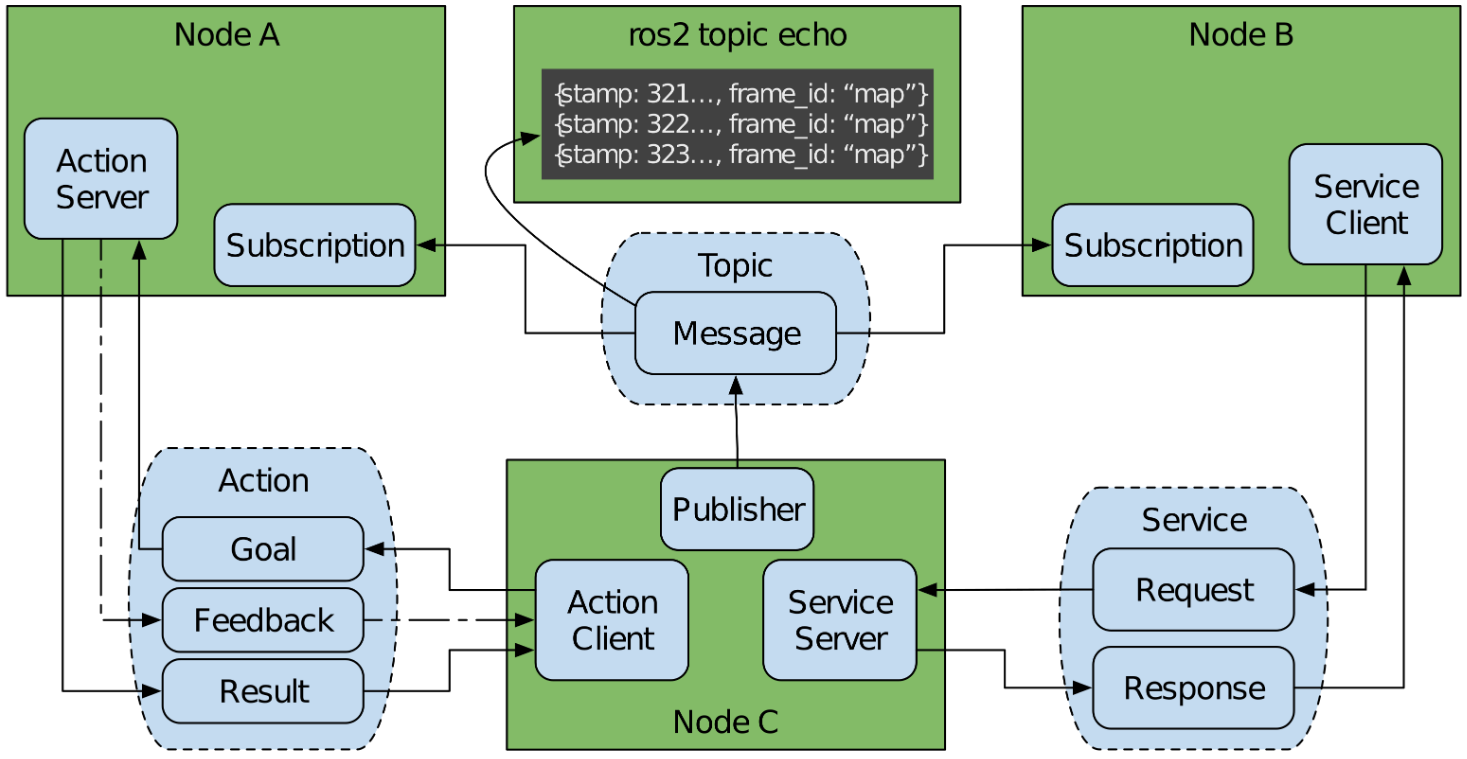
\includegraphics[width=1\textwidth]{Figures/c3/ros2_node_interfaces.png}
	\caption{Different communication patterns in \gls{ros2} organized under the \gls{node} interface \cite{macenski_robot_2022}.}
	\label{c3_fig_ros2_node_interfaces}
\end{figure}
It is an open source software development kit distributed under the Apache 2.0 License and can be split into three categories. The middleware, algorithms and developer tools \cite{macenski_robot_2022}. 
Written software can be divided thereby in dedicated parts, so-called \glspl{node}. In \gls{ros2} there is unified API which allows creating multiple communication patterns under the concept of \glspl{node}. This is represented in figure \ref{c3_fig_ros2_node_interfaces}. The most important concepts for this thesis are: \glspl{topic} and \glspl{service}. \Glspl{topic} provide an interface for passing \glspl{message} in an asynchronous manner. \Glspl{service} on the other hand, allow exchange of data in a request-response style pattern. Here, it is not mandatory that the client making the request blocks until the response arrives \cite{rico_concise_2022, macenski_robot_2022}.\newline
In figure \ref{c3_fig_ros2_stack} the client library API stack of \gls{ros2} is shown. \gls{ros2} follows earlier design philosophies and consists of several abstraction layers distributed across different packages. These layers allow multiple solutions for needed functions and allow users to replace components or select specific parts of the system that they need. Most users interact with the client libraries like \gls{rclcpp} and \gls{rclpy}. The \gls{rclcpp} and \gls{rclpy} libraries provide access to the main communication APIs and are tailored to specific programming languages. \gls{ros2} supports distributed computing on multiple machines and processes, including integration with cloud resources. It uses an intermediate interface called \gls{rcl} for common functions, and underneath, the middleware abstraction layer called \gls{rmw} provides key communication interfaces. Different \gls{rmw} implementations representing different middleware technologies can be used interchangeably depending on performance, licensing, or platform requirements \cite{rico_concise_2022, macenski_robot_2022, liao_introduction_2020}. \newline
The \gls{rmw} should be agnostic to \gls{dds} and the default middleware used in \gls{ros2} is eProsima's FastDDS \cite{macenski_robot_2022, noauthor_ros_nodate-1, noauthor_eprosima_nodate}. A more detailed introduction to \gls{dds} and to different implementations of \gls{dds} is given in section \ref{c3_sec_dds}.
\begin{figure}[htbp]
	\centering
	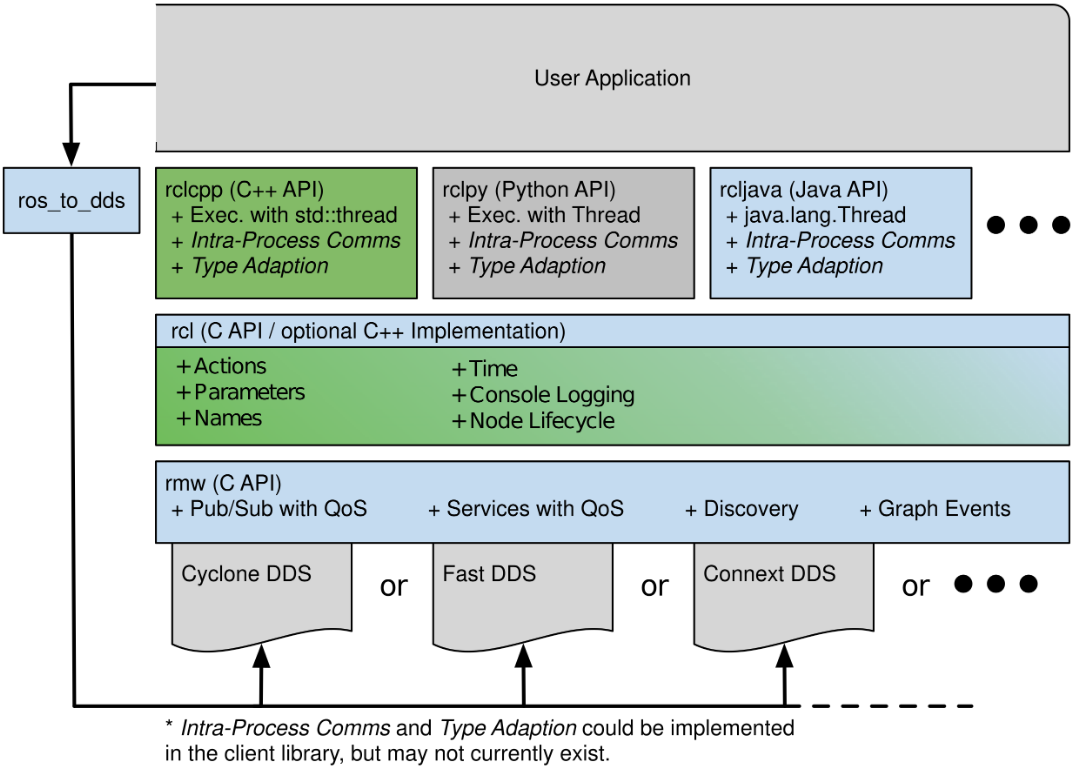
\includegraphics[width=1\textwidth]{Figures/c3/ros2_client_library_stack.png}
	\caption{The \gls{ros2} client library API stack with the support of different \gls{dds} implementations shown \cite{macenski_robot_2022}.}
	\label{c3_fig_ros2_stack}
\end{figure}

%%%%%%%%%%%%%%%%%%%%%%%%%%%%%%%%%%%%%%%%%%%%%%%%%
%   Data Exchange in Real-Time over Networks    %
%%%%%%%%%%%%%%%%%%%%%%%%%%%%%%%%%%%%%%%%%%%%%%%%%
\section{OMG Data Distribution Service}\label{c3_sec_dds}
The \glsentryfull{dds} is an open international middleware standard for real-time and embedded systems\cite{noauthor_data_nodate}. It is designed to facilitate efficient and reliable communication between distributed systems and devices in a wide range of industries.\newline 
\gls{dds} provides a data-centric publish-subscribe communication model, where data producers (publishers) publish data on specific topics, and data consumers (subscribers) can subscribe to those topics. The subscriber then receives the corresponding data via the topic. \gls{dds} ensures that the data is delivered reliably and in a timely manner to all interested subscribers. \cite{pardo-castellote_omg_2003, schlesselman_omg_2004}.

Some of the key features of \gls{dds} are listed below:\todo{rewrite!!!!}
\begin{itemize}
    \item \gls{qos}: \gls{dds} allows fine-grained control over various quality-of-service parameters to meet the specific requirements of different applications. \gls{qos} settings include reliability, bandwidth, delivery deadlines, and resource limits.

    \item Data-centricity: \gls{dds} focuses on the data itself, rather than the underlying transport or network infrastructure. It enables decoupling of data producers and consumers, allowing flexible and dynamic system configurations.

    \item Scalability: \gls{dds} supports both local and distributed systems, allowing seamless communication across multiple nodes, networks, or even geographically dispersed systems. It can handle large-scale deployments with high data rates and low latency.

    \item Interoperability: \gls{dds} promotes interoperability between different vendors and platforms. Applications built using \gls{dds} can communicate with each other regardless of the programming language, operating system, or hardware used, as long as they adhere to the \gls{dds} standard.

    \item Extensibility: \gls{dds} provides a modular and extensible architecture, allowing additional functionality and customizations to be added through optional extensions and profiles.

\end{itemize}
\subsection{DDS Vendors and Implementations}
For \gls{dds} exist a huge variety of different vendors and implementations. In table \ref{c3_tab_overview_rmw} an overview of different \gls{dds} implementations used as \gls{rmw} is given.
\subsubsection*{Fast \gls{dds}}
Fast \gls{dds} by eProsima is the default \gls{rmw} used since \gls{ros2} Foxy. It is at the time of writing still used as the default \gls{rmw} for \gls{ros2} Rolling. As the default \gls{rmw} it is fully supported and deployed under an Apache 2 license together with the binary releases. 
\subsubsection*{Cyclon \gls{dds}}
Cyclon \gls{dds} is an implementation of the 
\subsubsection*{Connext \gls{dds}}
Connext \gls{dds} is an implementation of the 
\subsubsection*{Zenoh}
Zenoh is a publisher, subscriber and query protocol by the Eclipse foundation.
\href{https://www.adlinktech.com/en/Zenoh}{Zenoh} 
\href{https://zenoh.io/blog/2021-03-23-discovery/}{Zenoh advatages} 

\begin{table}[htbp]
    \centering
\begin{tabular}{ |c|c|c|c| }
\hline
\multicolumn{4}{|c|}{Overview of the used \gls{rmw}s} \\
\hline
Product name & License & \gls{rmw} implementation & status  \\
\hline
\hline
eProsima Fast \gls{dds} & Apache 2 & rmw\_fastrtps\_cpp & 
    \begin{minipage}{4.2cm}
	    \vskip 8pt
		  Full support. \textbf{Default} \textbf{RMW}. Packaged with binary releases.
	    \vskip 8pt
	\end{minipage} \\\hline
 Eclipse Cyclone \gls{dds} & \begin{minipage}{2cm} \vskip 8pt Eclipse Public License v2.0 \vskip 8pt\end{minipage} & rmw\_cyclone\gls{dds}\_cpp & 
    \begin{minipage}{4.2cm}
	   \vskip 8pt
      Full support. Packaged with binary releases.\newline\newline
	   \vskip 8pt
	\end{minipage} \\\hline
 RTI Connext \gls{dds} & \begin{minipage}{2cm} \vskip 8pt commercial, research \vskip 8pt\end{minipage} & rmw\_connext\_cpp & 
    \begin{minipage}{4.2cm}
	   \vskip 8pt
		 Full support. Support included in binaries, but Connext installed separately.
	   \vskip 8pt
	\end{minipage} \\\hline\hline
  Eclipse Zenoh & Apache 2 & $-$ & \begin{minipage}{4.2cm}
	 \vskip 8pt
		 Via Zenoh bridge for \gls{dds}. \gls{dds} publisher/subscribers are mirrored and communication routed through Zenoh.
	 \vskip 8pt
	\end{minipage} \\\hline
\end{tabular}
    \caption{Overview of the different \glspl{rmw} used for comparison. Eclipse Zenoh is not a \gls{rmw} implementation, but there exists a plugin, called \texttt{zenoh-plugin-\gls{dds}}, which allows to route the \gls{dds} traffic through Zenoh.}\label{c3_tab_overview_rmw}
\end{table}

\section{Real-Time Capability of \gls{ros2}}
For a result to be valid in a real-time system, not only must the result be correct, but the time at which the result was generated is also important. Real-time systems can be divided into soft, firm and hard real-time. In a soft real-time system, the deadline can be exceeded within certain limits without causing fatal system conditions. In both fixed and hard real-time systems, the deadline must not be exceeded. The difference is that in firm real-time systems the current execution is aborted without fatal system conditions if the deadline is exceeded. In hard real-time systems, however, exceeding the deadline leads to fatal system conditions.\newline
As already described in section described in section \ref{c2_sec_control_over_network} Gutiérrez et al. conducted some experiments regarding the capabilities of \gls{ros2} to provide real-time communication. They concluded soft real-time to be possible, but not hard \cite{gutierrez_towards_2018}. In further investigations, Puck et al. even suggested hard real-time to be possible with the correct system configuration \cite{puck_performance_2021}. One important factor is the real-time capably of the underlying operating system and the used network stack.

\subsection{Preempt-RT}
Linux distributions like Ubuntu, are not real-time capable out of the box. Preempt-RT is a patch for the Linux kernel, commonly used to enhance the Linux kernel with real-time capabilities \cite{noauthor_realtimestart_nodate}. The kernel patch does not provide hard real-time, since those require a proof that the given deadlines are met. For a complex operating system like Ubuntu such proofs become unfeasible \cite{puck_distributed_2020}. However, the patch provides soft real-time capabilities by allowing preemption anywhere in the Linux kernel and additional features to improve scheduling determinism.

%%%%%%%%%%%%%%%%%%%%%%%%%%%%%%%%%
%   The ros2_control Framework  %
%%%%%%%%%%%%%%%%%%%%%%%%%%%%%%%%%
\section{The \gls{r2c} Framework}\label{ros2_control}
The open-source framework \gls{r2c}, is a framework for real-time control, initially released for \gls{ros2} Foxy. It is a rewrite of \gls{rc}, with the goal to simplify integration of new hardware and overcome some drawbacks present in \gls{rc} \cite{noauthor_welcome_nodate, magyar_getting_started_with_ros2_control_2021, magyar_ros2_control_the_future_of_ros_control_2021}. As shown in table \ref{c3_tab_r2c_repos} the framework comprises multiple repositories. It includes core functionality like management of controllers and hardware, as well as implementations of commonly used controllers. Besides, it provides low-level tools for control theory and real-time control. \newline
A more detailed view of the internals of the \gls{r2c} framework is presented in figure \ref{c3_fig_ros2_control_uml}. As can be seen, the framework includes a controller manager. The controller 
\begin{table}[htbp]
    \centering
\begin{tabular}{ |c|c| }
\hline
\multicolumn{2}{|c|}{\gls{r2c} repositories} \\
\hline
Repository & Description  \\
\hline
\hline
\href{https://github.com/ros-controls/ros2_control}{ros2\_control} 
 & \begin{minipage}{11cm}
	 \vskip 8pt
		 Core functionality like controller manager, resource manager, interfaces for hardware abstraction, and more.
	 \vskip 8pt
	\end{minipage}  \\
\href{https://github.com/ros-controls/ros2_controllers}{ros2\_controllers}  & \begin{minipage}{11cm}
	 \vskip 8pt
		 Collection of commonly and widely used controllers like forward command controller, joint trajectory, \dots
	 \vskip 8pt
	\end{minipage}  \\
\href{https://github.com/ros-controls/control_toolbox}{control\_toolbox}  & \begin{minipage}{11cm}
	 \vskip 8pt
		Control theory implementations (e.g. PID) used by controllers.
	 \vskip 8pt
	\end{minipage}  \\
\href{https://github.com/ros-controls/realtime_tools}{realtime\_tools}  & \begin{minipage}{11cm}
	 \vskip 8pt
		 Toolkit for real-time use. It includes e.g. real-time buffers and real-time publishers.
	 \vskip 8pt
	\end{minipage}  \\
\href{https://github.com/ros-controls/control_msgs}{control\_msgs}   & \begin{minipage}{11cm}
	 \vskip 8pt
		 Common messages used within the framework.
	 \vskip 8pt
	\end{minipage}  \\
\hline
\end{tabular}
    \caption{Overview of the repositories the \gls{r2c} framework includes.}
    \label{c3_tab_r2c_repos}
\end{table}
manager serves as entry-point for users and provides \gls{ros2} services through which the user can interact with the system. Additionally, it is responsible for managing the controllers and connects them to the abstracted hardware. The abstraction from the physical hardware and drivers is handled by the resource manager. The resource manager is part of the controller manager. Moreover, the resource manager stores and manages the hardware inside a resource storage. The hardware abstraction is done through interfaces (called \textit{hardware components}). These \textit{hardware components} can be divided into three groups:
\begin{itemize}
    \item Actuator (\texttt{ActuatorInterface}): Robotic hardware like motors, valves, and other simple 1-\gls{dof} actuators.
    \item Sensor (\texttt{SensorInterface}): Robotic hardware that can sens and measure physical properties of the environment.
    \item System (\texttt{SystemInterface}): Complex multi-\gls{dof} robotic hardware like an industrial robot.
\end{itemize}
 Finally, there is a collection of controllers inside the \texttt{ros2\_controllers} repositories. Controllers are the units responsible fore calculating a system's input. The input is thereby calculated based on the measured error between a reference value and the system's output.\newline
 In conclusion, the framework can roughly be divided into two parts. The first part includes the controllers and the second part embraces the hardware. The controller manager connects those parts and serves as an entry-point for users to interact with the system.

\subsection{The Link between Controllers and Hardware}\label{c3_sec_link_ctrl_hw}
A very important concept to understand for this thesis are the \gls{ci} and the \gls{si}. As shown in figure \ref{c3_fig_ros2_control_uml} in the middle above, the \gls{ci} and \gls{si} are located between the hardware site and the controller site of the \gls{r2c} framework. They abstract away from the hardware. The resource manager stores and manages them. \gls{si} grands access to the state of the component, while \gls{ci} additionally enables to write commands to a hardware component. If a controller wants to get access to the hardware, the resource manager creates so-called loans (\textit{LoanedCommandInterface} or \textit{LoanedStateInterface}). Those loaned interfaces are then passed to the controller. The controller can then read the state and write commands to the hardware via those loans.\newline
This whole concept is based on a \gls{sm} architecture. The drivers of the hardware allocate memory where the values of the \gls{ci} and \gls{si} are stored. A pointer to the allocated memory is then passed to the control site of the framework via the \gls{ci} and \gls{si}.
\begin{figure}[htbp]
	\centering
	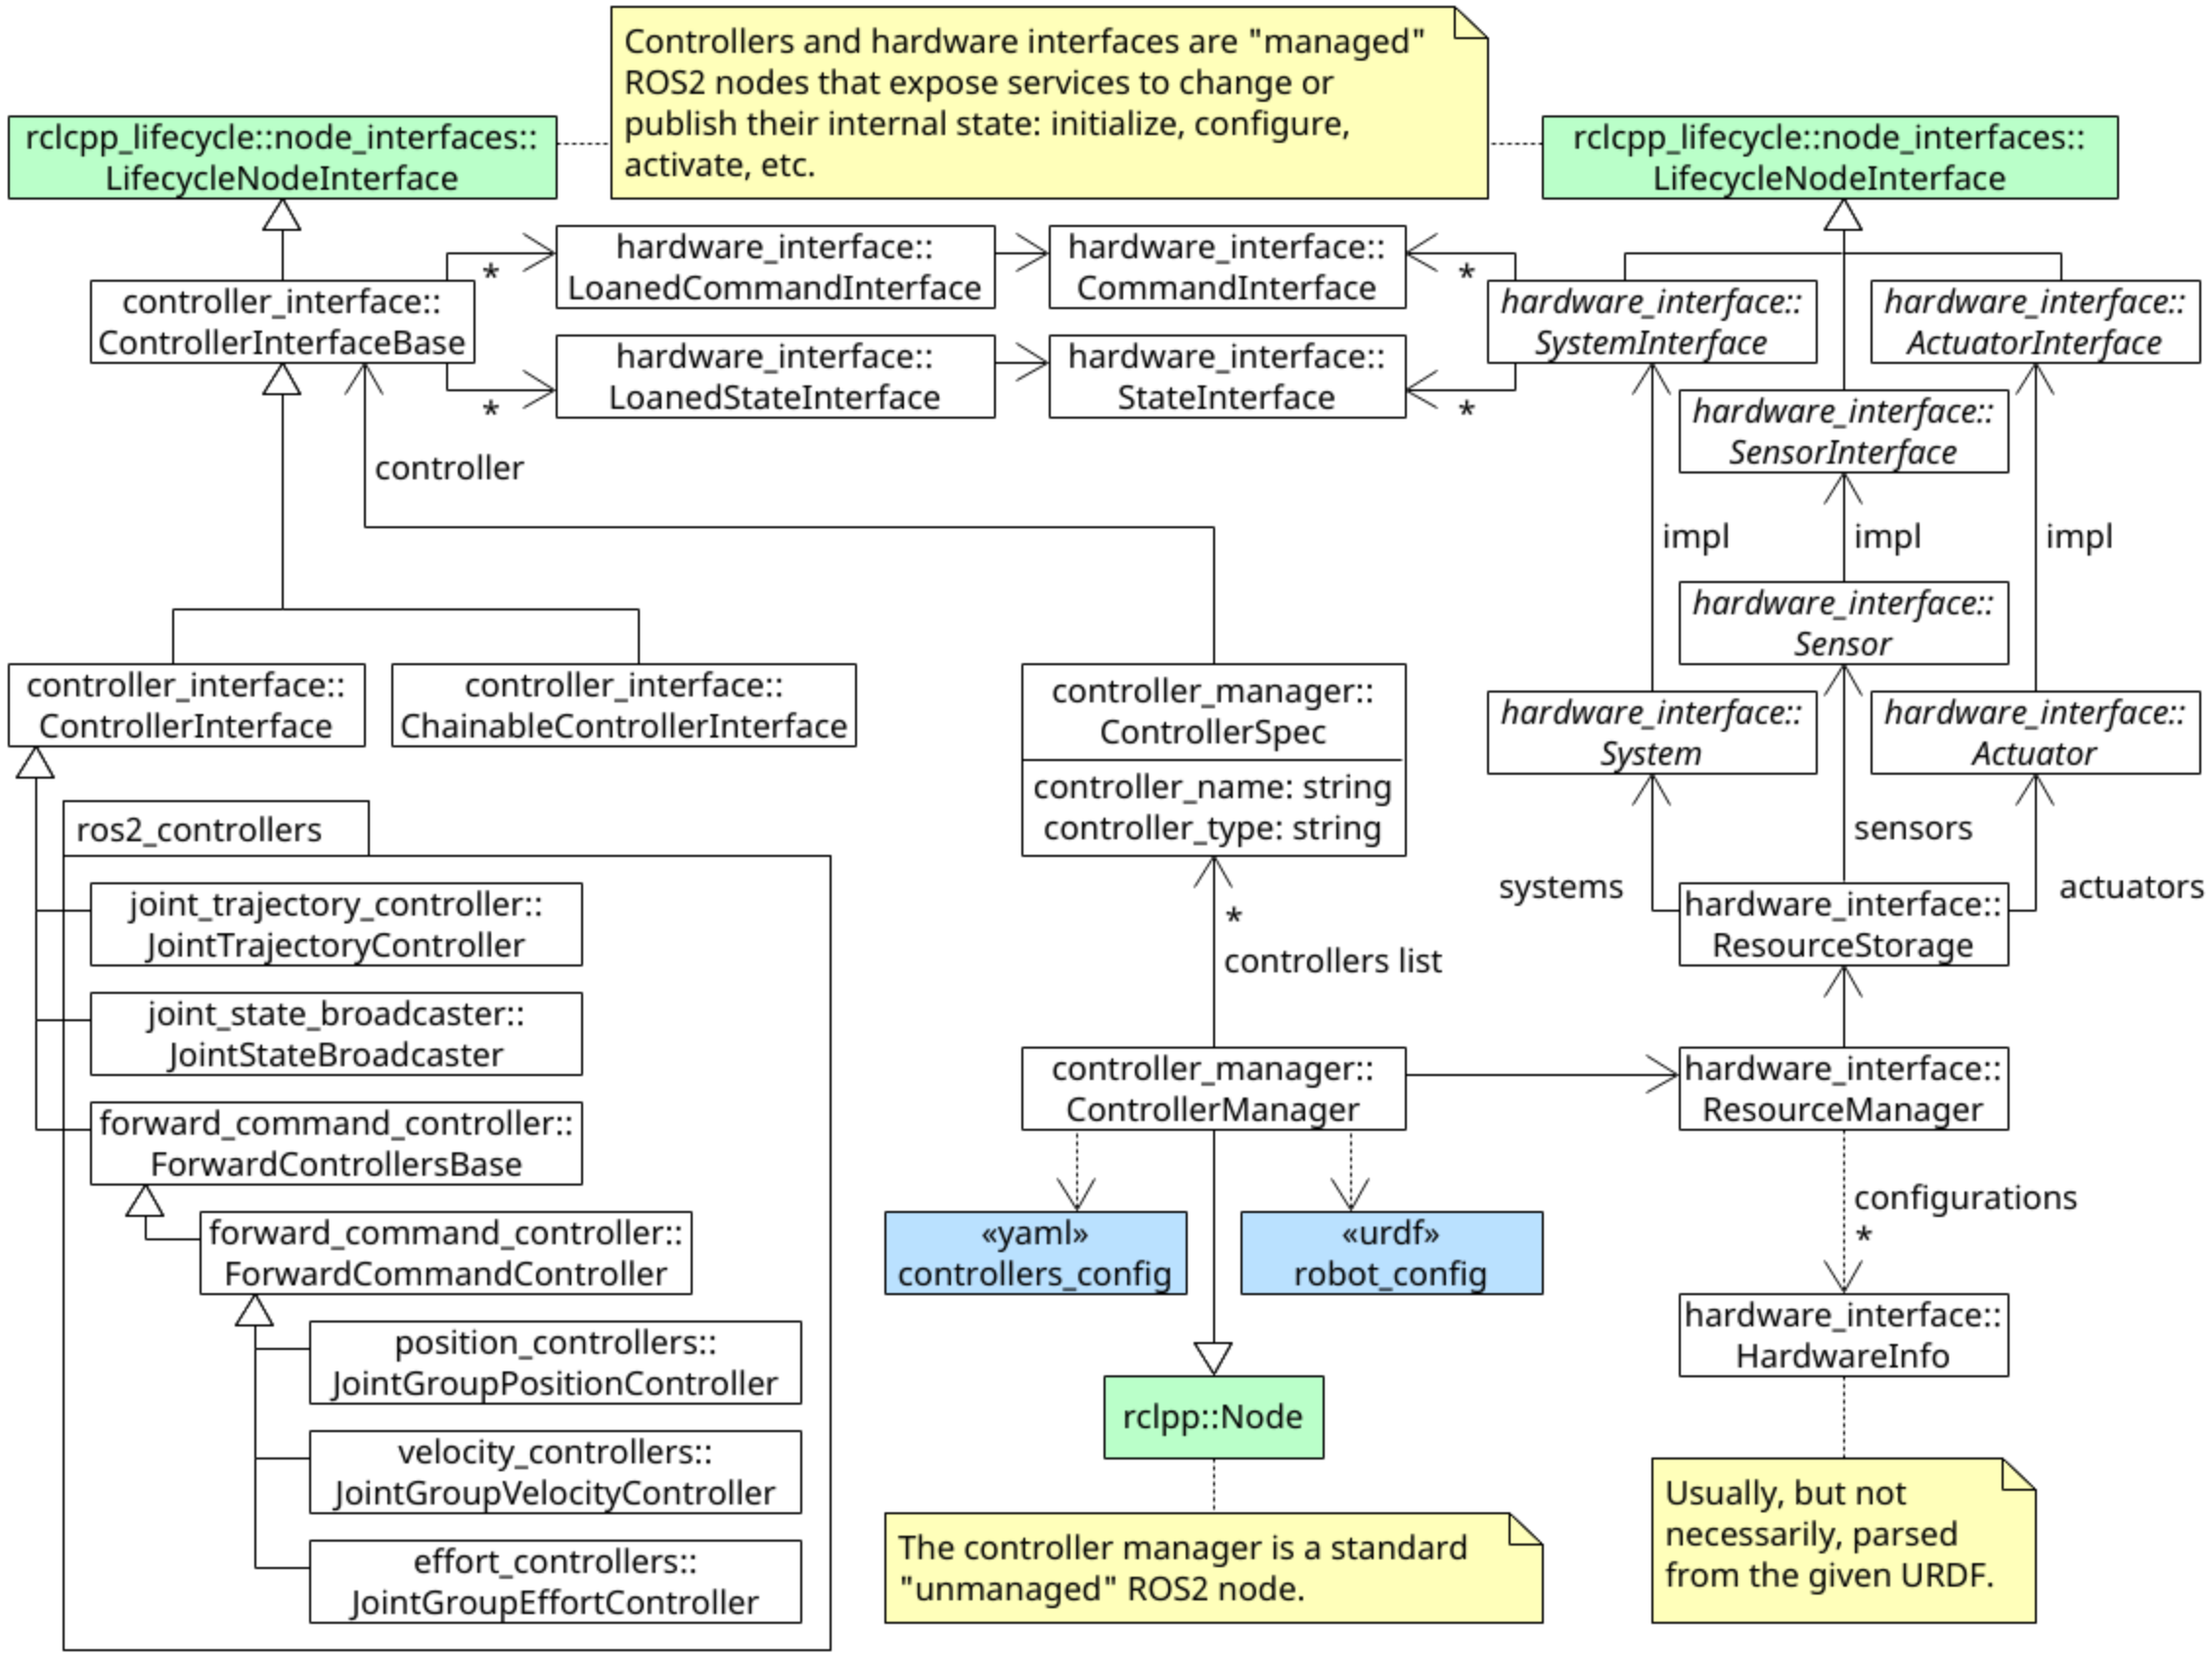
\includegraphics[width=1\textwidth]{Figures/c3/ros2_control_uml.png}
	\caption{UML diagram of the most important classes and interfaces in the \gls{r2c} framework. Picture taken from \cite{noauthor_welcome_nodate}. }
	\label{c3_fig_ros2_control_uml}
\end{figure}
 
\subsection{Controller Chaining}
Controller chaining in \gls{r2c} describes the possibility to link the output of one controller to the input of another. The chaining can thereby be in sequence (cascade control) or in parallel.\newline
For a controller to be able to be chained, it has to derive from the \textit{\seqsplit{ChainableController-Interface}}\todoBetter{Fix} instead of the \textit{ControllerInterface}. The chainable controller must then export reference interfaces. Those reference interfaces have the same meaning as the \textit{CommandInterfaces}. The controller can then run in either chained or external mode, where the latter is equivalent to a non chainable controller. If the controller runs in chained mode, all external interfaces like subscriber and services are disabled. This is done in order to avoid concurrency in the input commands. Another controller can then claim the reference interfaces and chain its output to the input of the chainable controller.
%  The control loop can be consist of three steps:
% \lstset{language=C++,basicstyle=\scriptsize}
% \begin{lstlisting}[caption=Pseudo code for the control loop.]
% // creat controller manager with an rclcpp::executor
% auto cm = 
%     std::make_shared<controller_manager::ControllerManager>(executor, cm_node_name);
% while (rclcpp::ok())
% {   
%     // calculated meassured_period
%     // execute update loop
%     cm->read(cm->now(), measured_period);
%     cm->update(cm->now(), measured_period);
%     cm->write(cm->now(), measured_period);
%     //sleep until next iteration
% }
% \end{lstlisting}\label{c3_code_control_loop}

\subsection{Controlling Multiple Robots with \gls{r2c}}\label{c3_sec_controlling_multiple_robots}
In the current state, \gls{r2c} focuses on controlling a single robot or robot cell. Further, the focus thereby lies on using a single computer to run the whole control stack. This includes the drivers used for communication with the hardware, the controller manager and controllers.\newline
Controlling multiple robots is however possible. Depending on the task, control of multiple robots in the current state of \gls{r2c} can roughly be split into two scenarios.
\begin{enumerate}[start=1,label={\upshape \texttt{Scenario \arabic*:}},wide = 0pt, leftmargin = 3em]
    \item Task where tight synchronization is needed. $\implies$ One platform with one controller manager. Represented in figure \ref{c3_fig_r2c_mr_ts}.
    \item Task where robots act more or less independent of one another. $\implies$ Multiple platforms with multiple independent controller managers. This can be seen in graphic \ref{c3_fig_r2c_mr_is}.
\end{enumerate}

\paragraph{Scenario 1:} 
In the first scenario, where a tight synchronization between the robots is needed, the most feasible way is to create on controller manager and multiple systems. One system for each robot. Each system can then be controlled by its own controller architecture. The controllers of those architectures are in turn managed by on controller manager. This controller manager can then handle the synchronization between the different systems.\newline
One should note, that this approach is limited to one machine. In the current form of \gls{r2c} there is no way to communicate between multiple controller managers. An outline of the architecture is given in representaion \ref{c3_fig_r2c_mr_ts}.
\begin{figure}[htbp]
	\centering
	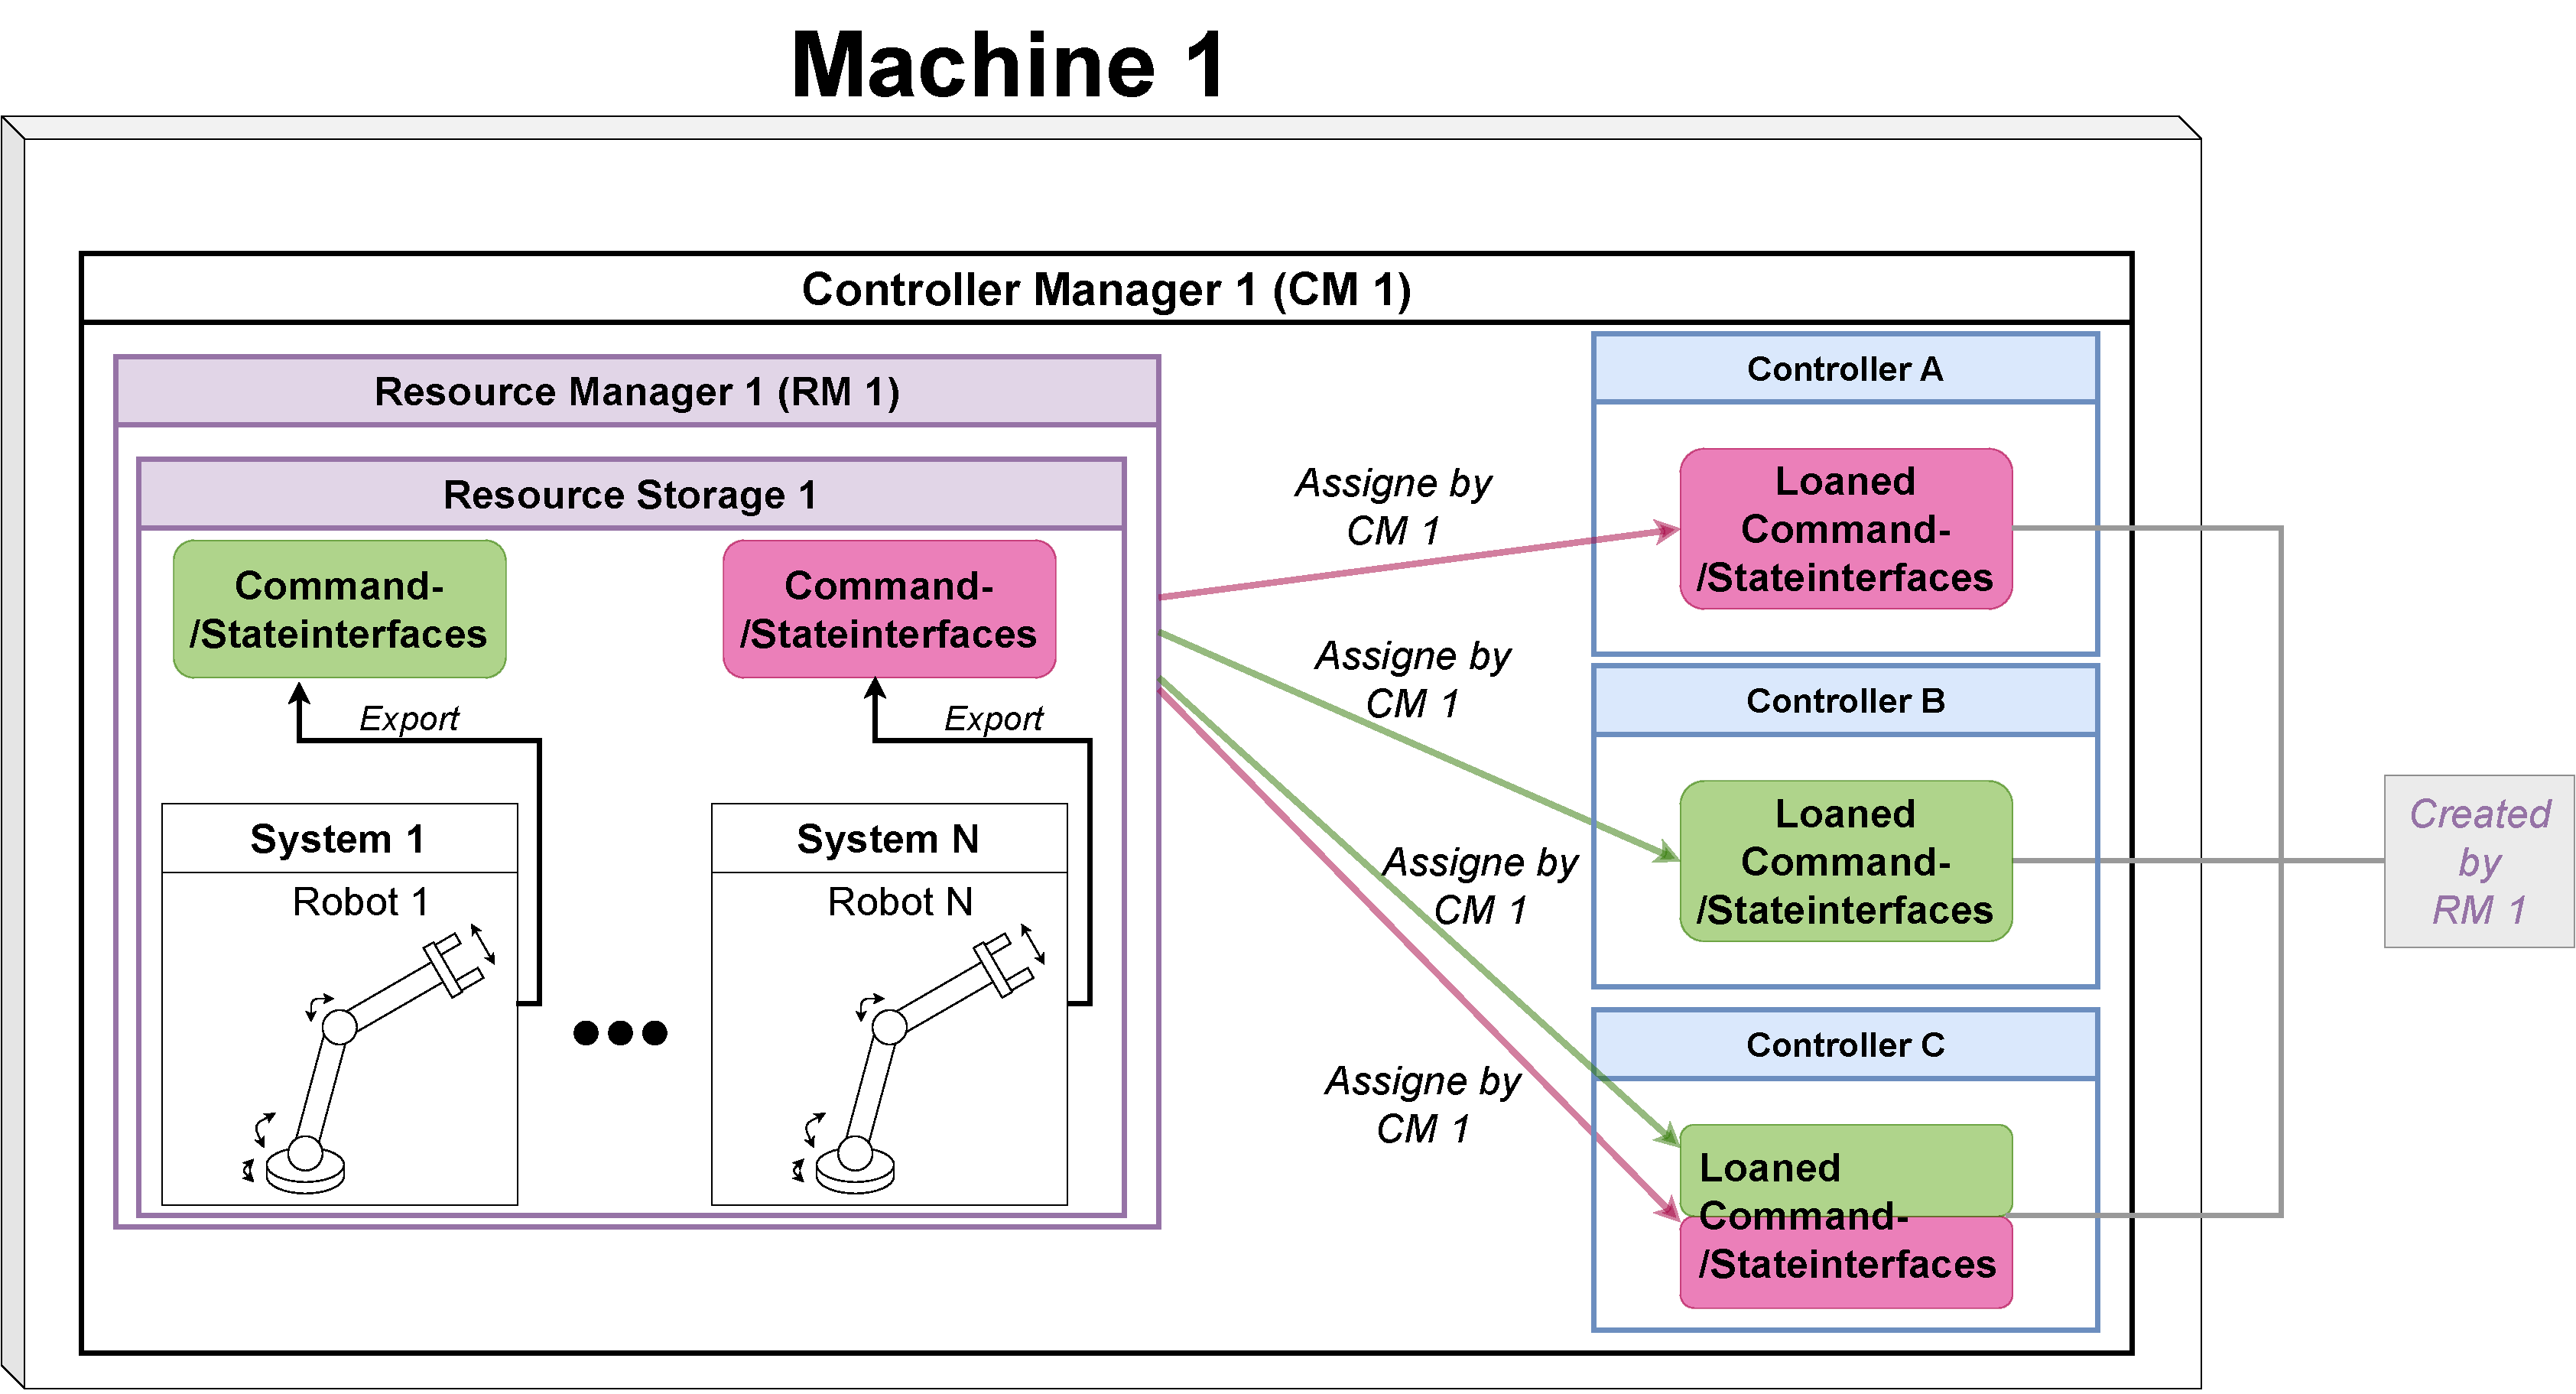
\includegraphics[width=1\textwidth]{Figures/c3/multiple_robots_one_system_current-Page-1.pdf}
	\caption{Schematic figure of how to realize a setup of multiple robots in \gls{r2c} where a tight synchronization between the robots is needed.}
	\label{c3_fig_r2c_mr_ts}
\end{figure}

\paragraph{Scenario 2:} 
In the second scenario, where no tight synchronization is needed and the robots act in a more or less independent manner, the most feasible way would be to have multiple machines with multiple controller managers running. Each controller manager would then have its own system. The system can then have its own controller architecture, which is managed by the corresponding controller manager. \newline
In this case, however, the systems are completely independent of each other. This means there is no synchronization between different systems possible. At least, there is no built-in functionality in \gls{r2c}. A schematic representation of this approach is provided in figure \ref{c3_fig_r2c_mr_is}.
\begin{figure}[htbp]
	\centering
	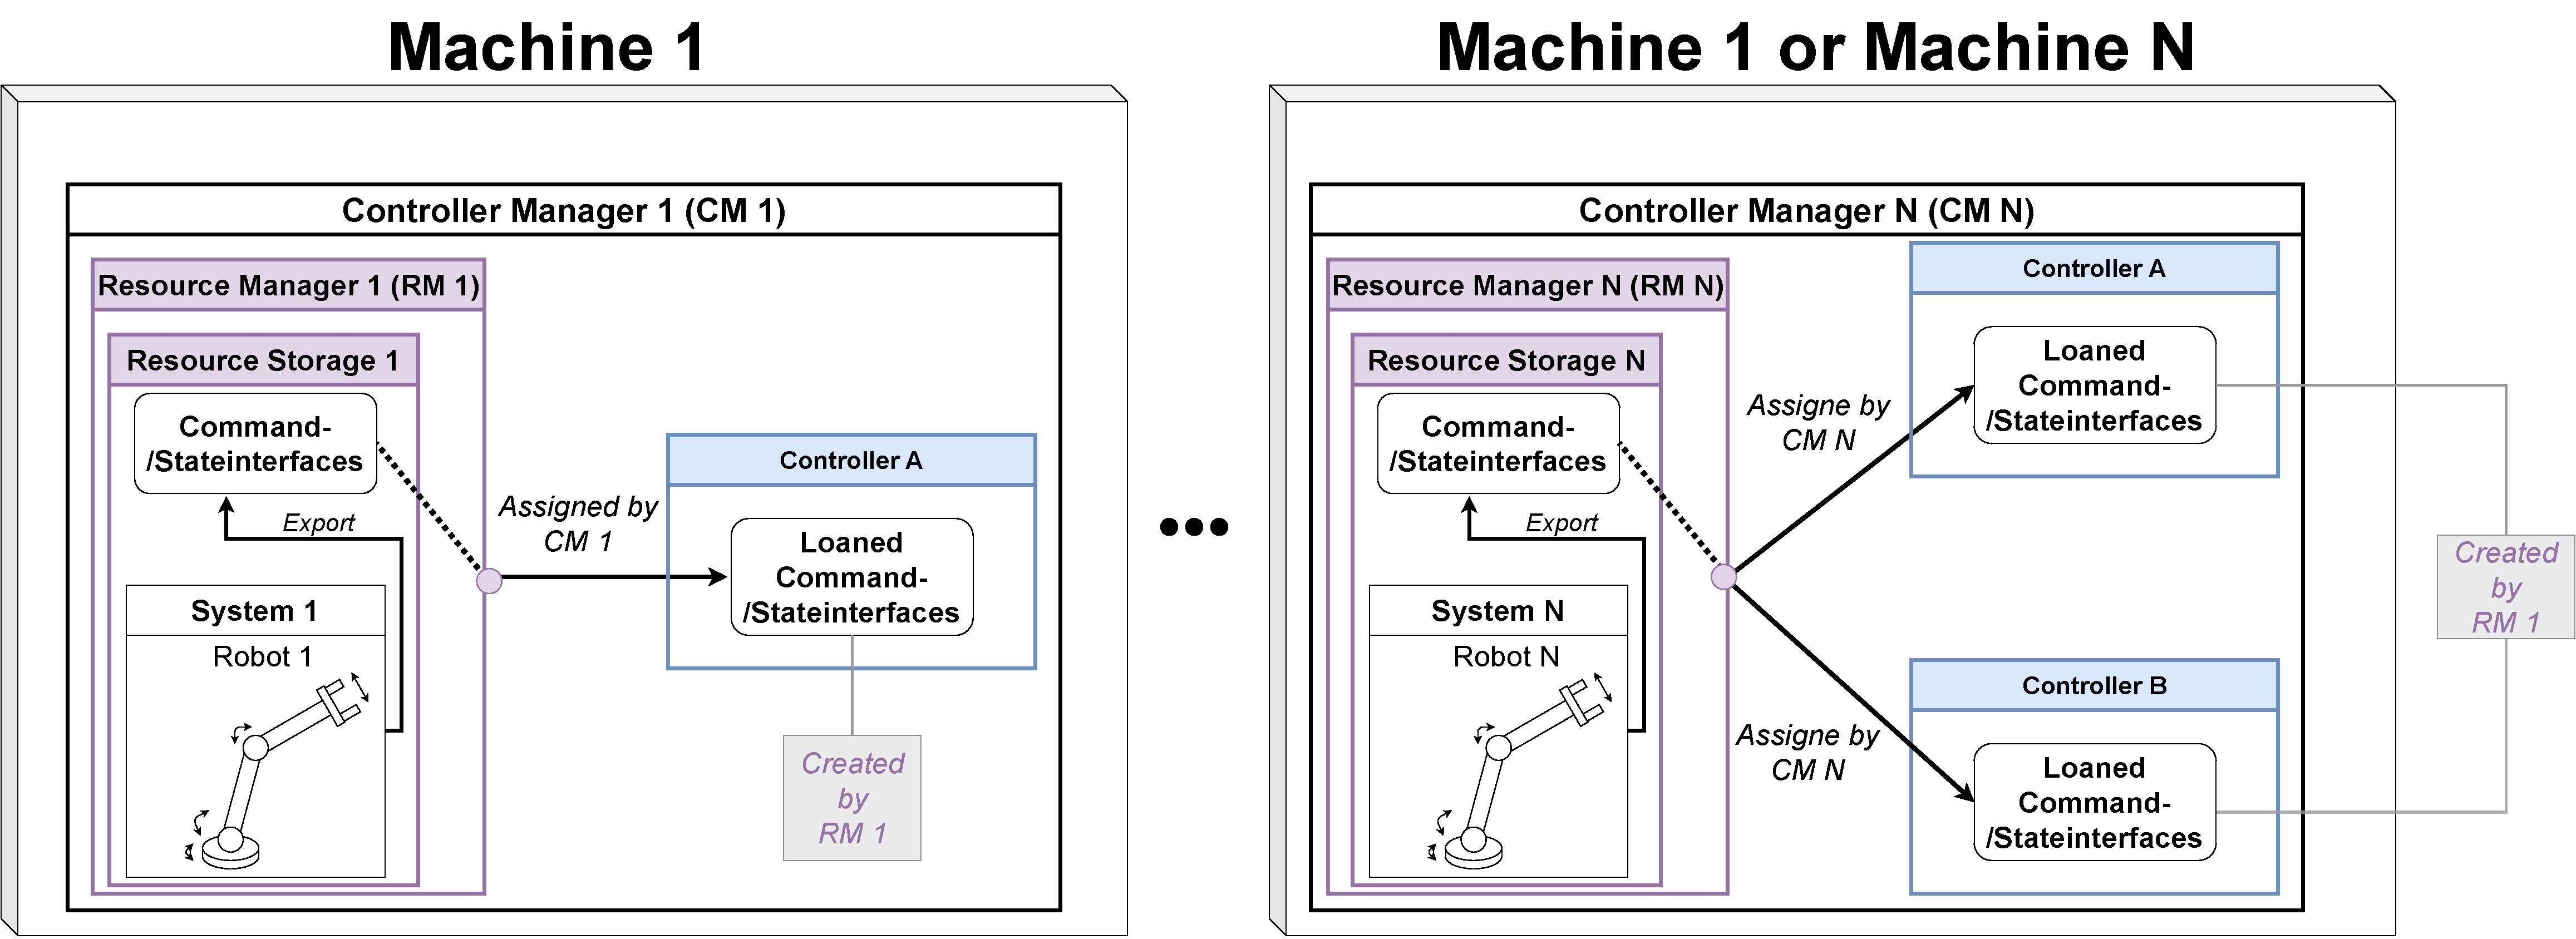
\includegraphics[width=1\textwidth]{Figures/c3/multiple_independent_robots_current.pdf}
	\caption{Schematic figure of how to realize a setup of multiple robots in \gls{r2c} where the robots act in an independent manner.}
	\label{c3_fig_r2c_mr_is}
\end{figure}





% \section{Time Synchronized Networks}
% What's the difference?????
% \section{Time Sensitive Networks}

\section{The Used Hardware}
\section{Computers}
Network card : lshw command
cpu : lscpu
memory: sudo dmidecode --type 17

\begin{table}[htbp]
    \centering
\begin{tabular}{ |c|c|c|c| }
\hline
\multicolumn{4}{|c|}{Overview of PCs used for the evaluation} \\
\hline
& PC1 & PC2 & PC3  \\
\hline
\hline
\textbf{Hardware} &  &  & \\\hline
    Processor &
        \begin{minipage}{3.7cm}
	       \vskip 8pt
		      16 $\times$ AMD Ryzen 7 5800H with Radeon Graphics
	       \vskip 8pt
	    \end{minipage} & 
        \begin{minipage}{3.7cm}
    	    \vskip 8pt
    		   16 $\times$ AMD Ryzen 7 5800H with Radeon Graphics
    	    \vskip 8pt
	    \end{minipage} & 
        \begin{minipage}{3.7cm}
	       \vskip 8pt
		      16 $\times$ AMD Ryzen 7 5800H with Radeon Graphics
	       \vskip 8pt
	    \end{minipage} \\\hline
    RAM &
        \begin{minipage}{3.7cm}
	       \vskip 8pt
		      2 $\times$ 32GB DDR4 Samsung SODIMM 3200 MT/s
	       \vskip 8pt
	    \end{minipage} & 
        \begin{minipage}{3.7cm}
    	    \vskip 8pt
    		   2 $\times$ 32GB DDR4 Samsung SODIMM 3200 MT/s
    	    \vskip 8pt
	    \end{minipage} & 
        \begin{minipage}{3.7cm}
	       \vskip 8pt
		      2 $\times$ 32GB DDR4 Samsung SODIMM 3200 MT/s
	       \vskip 8pt
	    \end{minipage} \\\hline
    Network Card &
        \begin{minipage}{3.7cm}
	       \vskip 8pt
		      Realtek Semiconductor Co., LtdRTL8125 2.5GbE Controller
	       \vskip 8pt
	    \end{minipage} & 
        \begin{minipage}{3.7cm}
    	    \vskip 8pt
    		   Realtek Semiconductor Co., LtdRTL8125 2.5GbE Controller
    	    \vskip 8pt
	    \end{minipage} & 
        \begin{minipage}{3.7cm}
          \vskip 8pt
		      Realtek Semiconductor Co., LtdRTL8125 2.5GbE Controller
	       \vskip 8pt
	    \end{minipage} \\\hline\hline
\textbf{Setup} & & & \\\hline
    Operating System & Kubuntu 22.04 &  Ubuntu 22.04 & Ubuntu 22.04 \\\hline
    Kernel &
        \begin{minipage}{3.7cm}
	       \vskip 8pt
		      A
	       \vskip 8pt
	    \end{minipage} & 
        \begin{minipage}{3.7cm}
    	   \vskip 8pt
    		   B
    	   \vskip 8pt
	    \end{minipage} & 
        \begin{minipage}{3.7cm}
	       \vskip 8pt
		      C
	       \vskip 8pt
	    \end{minipage} \\\hline
    Real-time Kernel &
        \begin{minipage}{3.7cm}
	       \vskip 8pt
    		   A
    	   \vskip 8pt
	    \end{minipage} & 
        \begin{minipage}{3.7cm}
    	   \vskip 8pt
    		   B
    	   \vskip 8pt
	    \end{minipage} & 
        \begin{minipage}{3.7cm}
    	   \vskip 8pt
    		   C
    	   \vskip 8pt
	    \end{minipage} \\\hline
    ROS version & Rolling & Rolling & Rolling \\\hline
        \begin{minipage}{3cm}
        \vskip 4pt
    		   ros2\_control based on commit:\vskip 8pt
	    \end{minipage} & 0eb319ea43b78b886a & 0eb319ea43b78b886a & 0eb319ea43b78b886a \\\hline
            \begin{minipage}{3cm}
        \vskip 4pt
    		   ros2\_controllers based on commit:\vskip 8pt
	    \end{minipage} & 05d7a5ec73a02eab2c & 05d7a5ec73a02eab2c & 05d7a5ec73a02eab2c \\\hline
\end{tabular}
    \caption{Three different computers were used for the evaluation. The table gives an overview of the used hardware, as well as the setup on each of the computers.}
    \label{c3_tab_r2c_repos}
\end{table}
\subsection{Robots for Evaluation}
The used robots for the evaluation are the KUKA KR 3 R540 \cite{noauthor_agile_nodate, noauthor_kuka_kr_3_agiluspdf_nodate}





%% ==============================
\chapter{\iflanguage{ngerman}{Konzept}{Concept}}
\label{sec:concept}
%% ==============================

\section{Conceptual Design}
As described in section \ref{c3_sec_controlling_multiple_robots} in the current state of \gls{r2c} the control of multiple robots is only possible in two ways. Either on one machine with a tight synchronization or on multiple machines with no significant synchronization at all. The goal of this work is to test whether it is possible in the \gls{r2c} context to run multiple controllers on multiple machines and still allow tight synchronization.\newline
As shown in the UML class diagram in graphic \ref{c3_fig_ros2_control_uml} the link between the hardware site and the controllers in the \gls{r2c} framework are the \texttt{CommandInterfaces} and the \texttt{StateInterfaces}. See section \ref{c3_sec_link_ctrl_hw} for a more detailed explanation of the conceptual background.\newline
\begin{figure}[htbp]
	\centering

 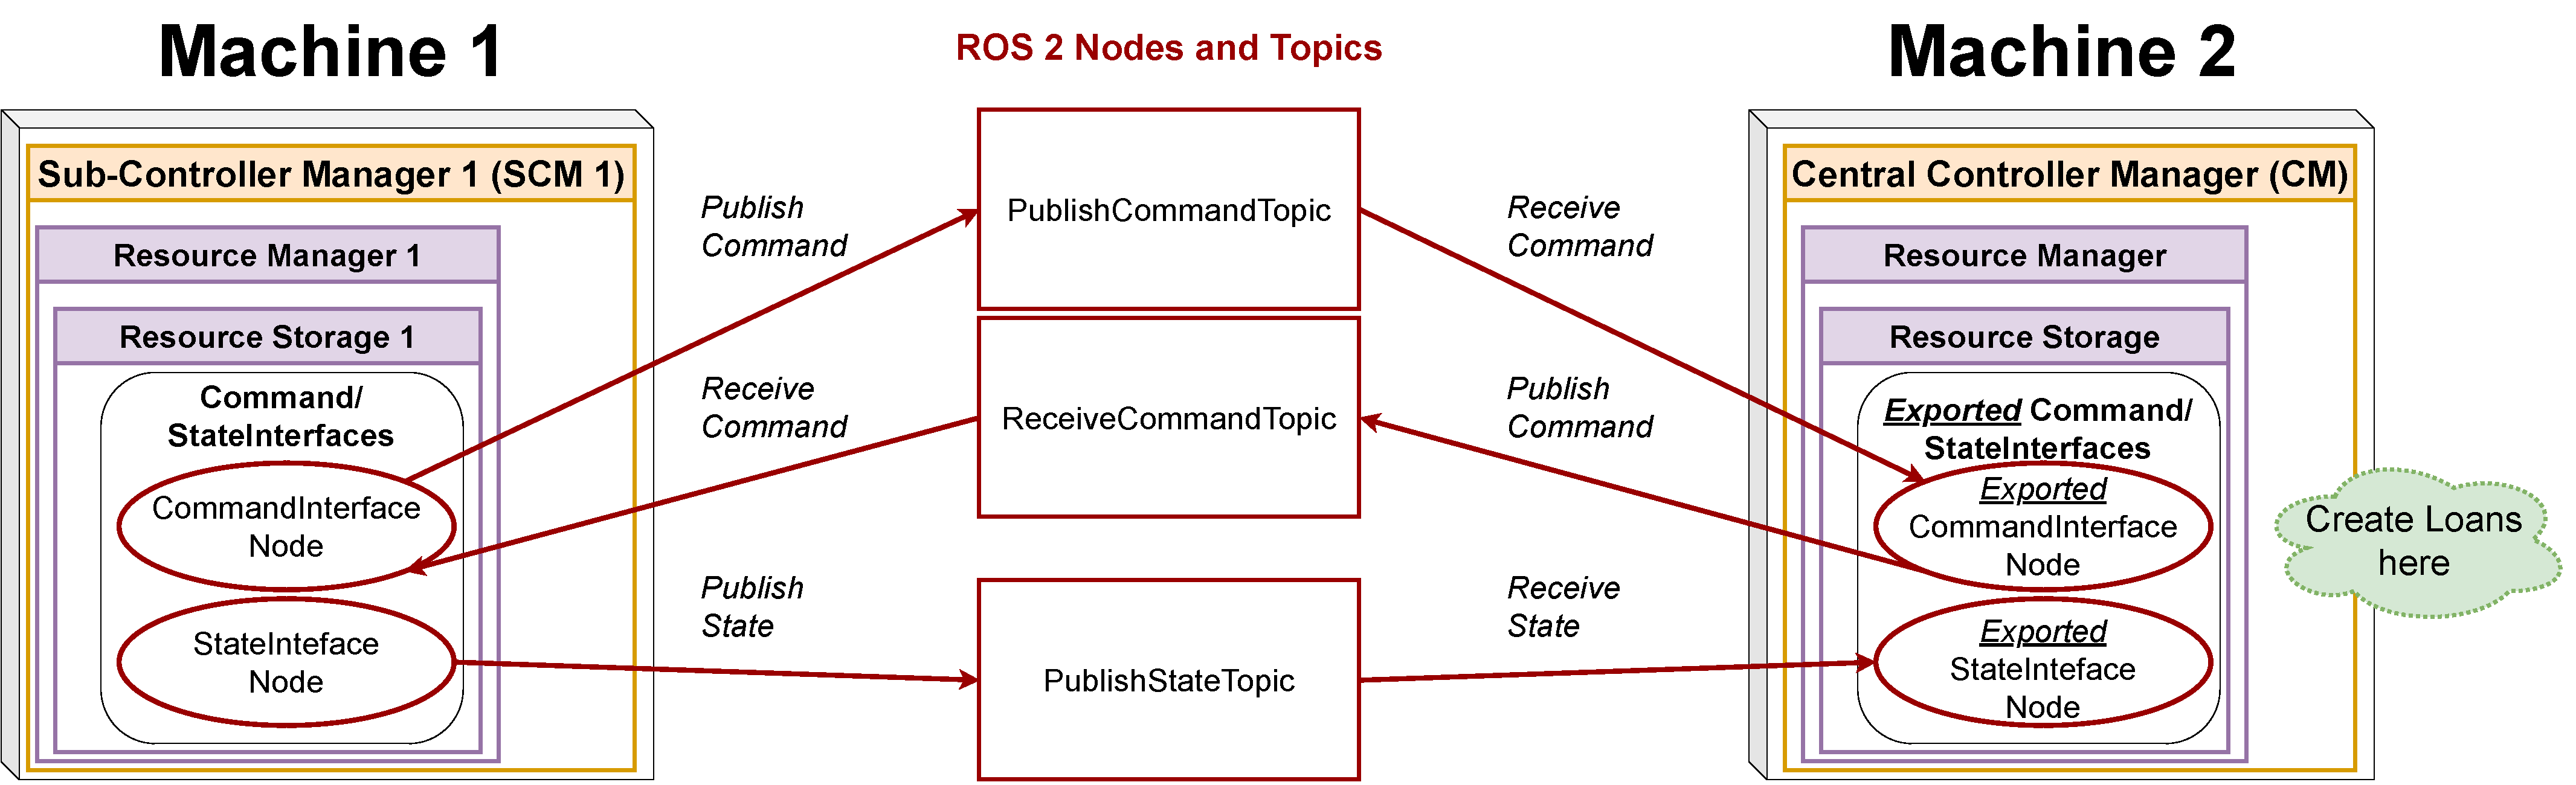
\includegraphics[width=1\textwidth]{Figures/C4/simple_concept.drawio.pdf}
	\caption{Schematic overview of the concept implemented.}
	\label{c4_fig_simple_concept}
\end{figure}
The fundamental idea of the design is to split the system at this point. 




\section{Integration in \gls{r2c}}

\subsection{Central Controller Manager}
\begin{itemize}
    \item \textbf{Subcontroller manager:}
    \begin{itemize}
        \item register subcontroller manager $\implies$ export descriptions of Command-/SystemInterfaces
        \item create publisher for Command-/StateInterfaces
        \item wait for registration to successfully complete
        \item subscribe to commandpublisher received from central controller manager
    \end{itemize}
    \item \textbf{Central Controller manager:}
    \begin{itemize}
        \item create service for registration
        \item register subcontroller manger if receive call
        \item subscribe to publisher of Command-/StateInteface of subcontrolelr manager
        \item create special Command-/StateInterfaces for this
        \item create publisher for Commands
        \item proceed as normal
    \end{itemize}
\end{itemize}
\begin{figure}[htbp]
	\centering
	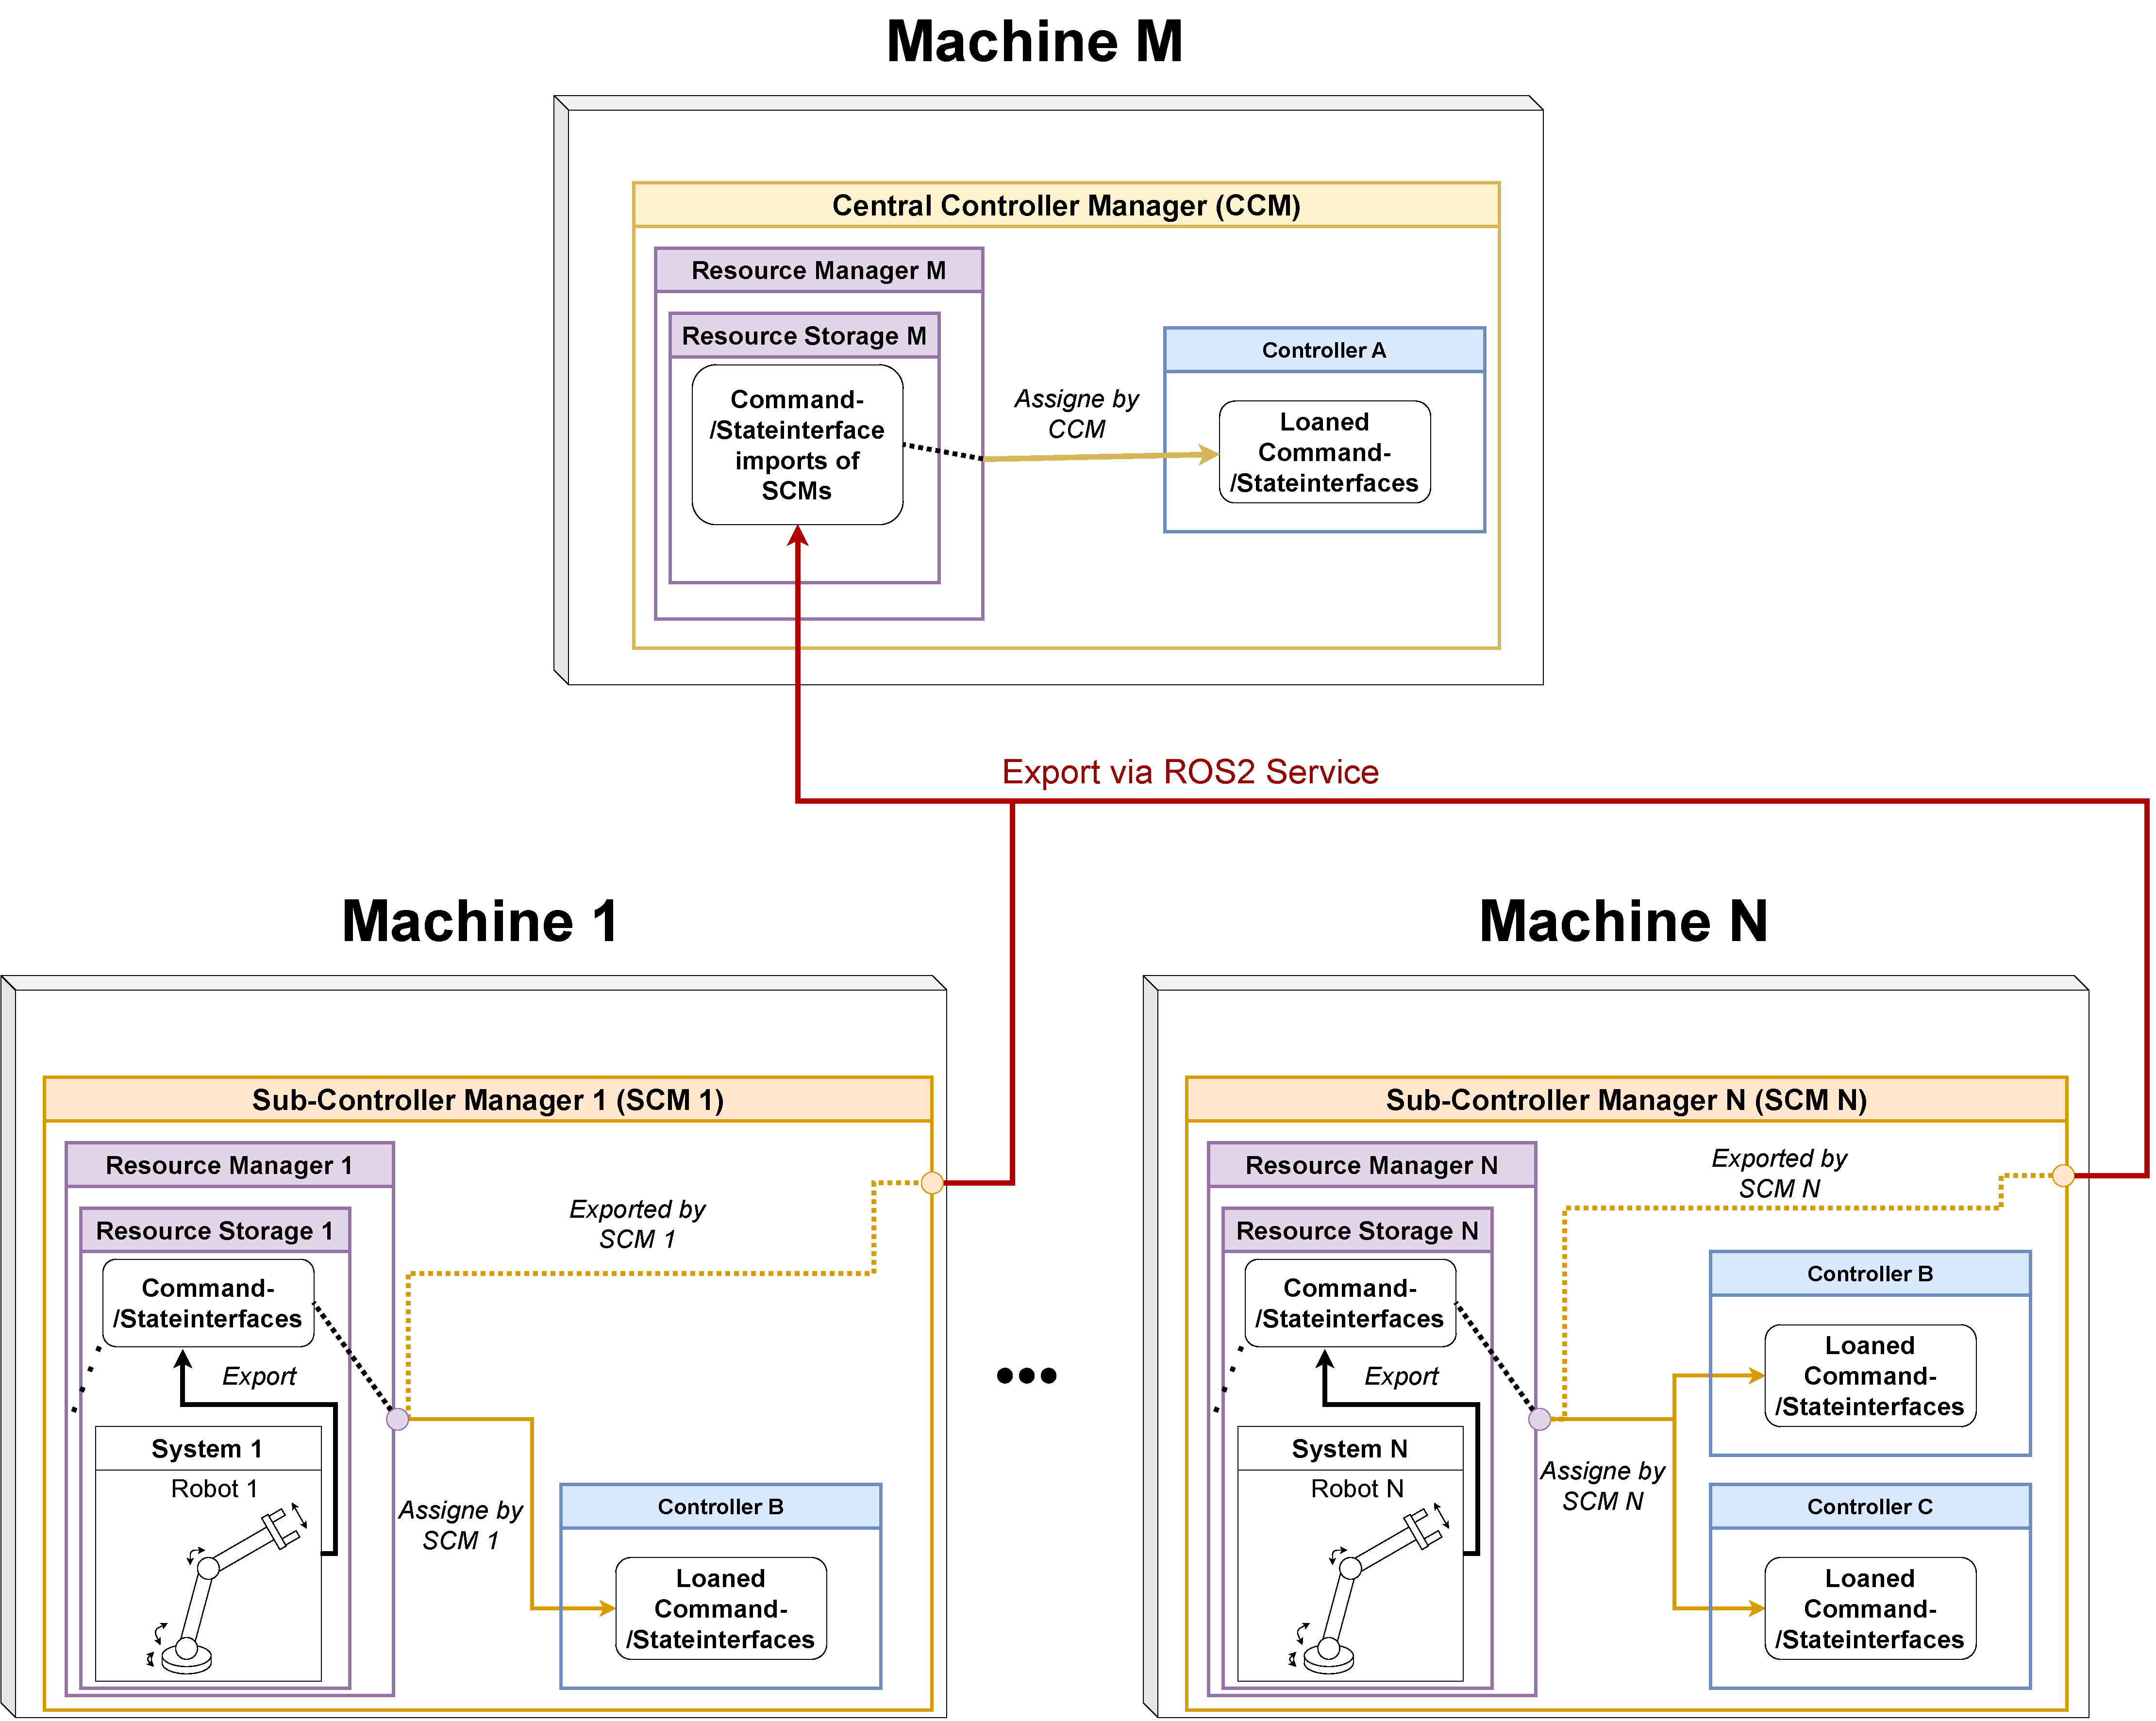
\includegraphics[width=1\textwidth]{Figures/C4/distributed_control.drawio.pdf}
	\caption{Schematic overview of the concept implemented.}
	\label{c4_fig_concept_overview}
\end{figure}

\subsection{Controller Chaining}
\begin{itemize}
    \item \textbf{Subcontroller manager:}
    \begin{itemize}
        \item same as for simple case
        \item export additionally reference interfaces
    \end{itemize}
    \item \textbf{Central Controller manager:}
    \begin{itemize}
        \item same as simple case
        \item import reference interfaces
        \item create chained controller
        \item proceed as normal
    \end{itemize}
\end{itemize}
%% ==============================
% Part is used only in PhD thesis
\part{The Implementation}
\chapter{\iflanguage{ngerman}{Implementierung}{Implementation}}
\label{sec:implementation}

\section{Porting of the KUKA RSI to \gls{ros2} Rolling}
The concept should later be tested with real hardware at the \gls{kit} \gls{ipr}. The used hardware are KUKA robots. The \gls{rsi} was only available for older versions of \gls{ros} and needed to be ported.\newline


Creation of Hardware to run UDP server and creation of control node. Ignore controller manager's update rate. Synchronization via blocking read() timing issues. Usage of a steady clock.

\section{Preparation Work}

\subsection{Allow to Start with Empty Robot Description File}

\subsection{Publish Robot Description File}

\subsection{Adaption of Handles}

\section{Controller Manager Hierachie}
\subsection{Central Controller Manager}
\subsubsection{Configuration of a Central Controller Manager}
\lstset{language=yaml,basicstyle=\scriptsize}
\begin{lstlisting}[caption=Example configuration of a central controller manager with a joint trajecotry controller.]
controller_manager:
  ros__parameters:
    central_controller_manager: true
    
    position_trajectory_controller:
      type: joint_trajectory_controller/JointTrajectoryController

position_trajectory_controller:
  ros__parameters:
    joints:
      - /sub_1/sub_1_joint_a1
      - /sub_1/sub_1_joint_a2
      - /sub_1/sub_1_joint_a3
      - /sub_1/sub_1_joint_a4
      - /sub_1/sub_1_joint_a5
      - /sub_1/sub_1_joint_a6
      - /sub_2/sub_2_joint_a1
      - /sub_2/sub_2_joint_a2
      - /sub_2/sub_2_joint_a3
      - /sub_2/sub_2_joint_a4
      - /sub_2/sub_2_joint_a5
      - /sub_2/sub_2_joint_a6

    command_interfaces:
      - position

    state_interfaces:
      - position
    ... # Some configuration for JointTrajectoryController 
\end{lstlisting}\label{c5_l_central_controller_manager_config}

\subsubsection{Configuration of a Chained Central Controller Manager}
\lstset{language=yaml,basicstyle=\scriptsize}
\begin{lstlisting}[caption=Example configuration of a chained central controller manager.]
controller_manager:
  ros__parameters:
    central_controller_manager: true

    fpc_jtc_chain_controller:
      type: forward_command_controller/ForwardCommandController

fpc_jtc_chain_controller:
  ros__parameters:
    joints:
      - /sub_1/position_trajectory_controller/sub_1_joint_a1
      - /sub_1/position_trajectory_controller/sub_1_joint_a2
      - /sub_1/position_trajectory_controller/sub_1_joint_a3
      - /sub_1/position_trajectory_controller/sub_1_joint_a4
      - /sub_1/position_trajectory_controller/sub_1_joint_a5
      - /sub_1/position_trajectory_controller/sub_1_joint_a6
      - /sub_2/position_trajectory_controller/sub_2_joint_a1
      - /sub_2/position_trajectory_controller/sub_2_joint_a2
      - /sub_2/position_trajectory_controller/sub_2_joint_a3
      - /sub_2/position_trajectory_controller/sub_2_joint_a4
      - /sub_2/position_trajectory_controller/sub_2_joint_a5
      - /sub_2/position_trajectory_controller/sub_2_joint_a6
    interface_name: position
\end{lstlisting}\label{c5_l_chained_central_controller_manager_config}

\subsection{Sub-Controller Manager}

\subsection{Configuration of a Sub-Controller Manager}
\lstset{language=yaml,basicstyle=\scriptsize}
\begin{lstlisting}[caption=Example configuration of a sub-controller manager which exports all of it's command and state interfaces.]
/sub_1/controller_manager:
  ros__parameters:
    update_rate: 10  # Hz
    sub_controller_manager: true
    distributed_interfaces_publish_period: 4 # ms
\end{lstlisting}\label{c5_l_sub_controller_manager_config}
\lstset{language=yaml,basicstyle=\scriptsize}

\subsection{Configuration of a Chained Sub-Controller Manager}
\begin{lstlisting}[caption=Example configuration of a chained sub-controller manager.]
/sub_1/controller_manager:
  ros__parameters:
    update_rate: 10  # Hz
    sub_controller_manager: true
    distributed_interfaces_publish_period: 4
    export_command_interfaces:
      - ""  # don't export any command interfaces
    export_state_interfaces:
      - "" # don#t export any state intefaces

    position_trajectory_controller:
      type: joint_trajectory_controller/JointTrajectoryController

/sub_1/position_trajectory_controller:
  ros__parameters:
    joints:
      - sub_1_joint_a1
      - sub_1_joint_a2
      - sub_1_joint_a3
      - sub_1_joint_a4
      - sub_1_joint_a5
      - sub_1_joint_a6

    command_interfaces:
      - position

    state_interfaces:
      - position
   ... # Some configuration for JointTrajectoryController 
\end{lstlisting}\label{c5_l_chained_sub_controller_manager_config}
%% ==============================
\chapter{\iflanguage{ngerman}{Ergebnisse}{Results}}
\label{sec:results}
%% ==============================
\section{Experimental Setup for Evaluation}
Network card : lshw command
cpu : lscpu
memory: sudo dmidecode --type 17

\begin{table}[htbp]
    \centering
\begin{tabular}{ |c|c|c|c| }
\hline
\multicolumn{4}{|c|}{Overview of PCs used for the evaluation} \\
\hline
& PC1 & PC2 & PC3  \\
\hline
\hline
\textbf{Hardware} &  &  & \\\hline
    Processor &
        \begin{minipage}{3.9cm}
	       \vskip 8pt
		      16 $\times$ AMD Ryzen 7 5800H with Radeon Graphics
	       \vskip 8pt
	    \end{minipage} & 
        \begin{minipage}{3.9cm}
    	    \vskip 8pt
    		   16 $\times$ AMD Ryzen 7 5800H with Radeon Graphics
    	    \vskip 8pt
	    \end{minipage} & 
        \begin{minipage}{3.9cm}
	       \vskip 8pt
		      16 $\times$ AMD Ryzen 7 5800H with Radeon Graphics
	       \vskip 8pt
	    \end{minipage} \\\hline
    RAM &
        \begin{minipage}{3.9cm}
	       \vskip 8pt
		      2 $\times$ 32GB DDR4 Samsung SODIMM 3200 MT/s
	       \vskip 8pt
	    \end{minipage} & 
        \begin{minipage}{3.9cm}
    	    \vskip 8pt
    		   2 $\times$ 32GB DDR4 Samsung SODIMM 3200 MT/s
    	    \vskip 8pt
	    \end{minipage} & 
        \begin{minipage}{3.9cm}
	       \vskip 8pt
		      2 $\times$ 32GB DDR4 Samsung SODIMM 3200 MT/s
	       \vskip 8pt
	    \end{minipage} \\\hline
    Network Card &
        \begin{minipage}{3.9cm}
	       \vskip 8pt
		      Realtek Semiconductor Co., LtdRTL8125 2.5GbE Controller
	       \vskip 8pt
	    \end{minipage} & 
        \begin{minipage}{3.9cm}
    	    \vskip 8pt
    		   Realtek Semiconductor Co., LtdRTL8125 2.5GbE Controller
    	    \vskip 8pt
	    \end{minipage} & 
        \begin{minipage}{3.9cm}
          \vskip 8pt
		      Realtek Semiconductor Co., LtdRTL8125 2.5GbE Controller
	       \vskip 8pt
	    \end{minipage} \\\hline\hline
\textbf{Setup} & & & \\\hline
    Operating System & Kubuntu 22.04 &  Ubuntu 22.04 & Ubuntu 22.04 \\\hline
    Kernel &
        \begin{minipage}{3.9cm}
	       \vskip 8pt
		      A
	       \vskip 8pt
	    \end{minipage} & 
        \begin{minipage}{3.9cm}
    	   \vskip 8pt
    		   B
    	   \vskip 8pt
	    \end{minipage} & 
        \begin{minipage}{3.9cm}
	       \vskip 8pt
		      C
	       \vskip 8pt
	    \end{minipage} \\\hline
    Real-time Kernel &
        \begin{minipage}{3.9cm}
	       \vskip 8pt
    		   A
    	   \vskip 8pt
	    \end{minipage} & 
        \begin{minipage}{3.9cm}
    	   \vskip 8pt
    		   B
    	   \vskip 8pt
	    \end{minipage} & 
        \begin{minipage}{3.9cm}
    	   \vskip 8pt
    		   C
    	   \vskip 8pt
	    \end{minipage} \\\hline
    ROS version & Rolling & Rolling & Rolling \\\hline
        \begin{minipage}{3cm}
        \vskip 4pt
    		   ros2\_control based on commit:\vskip 8pt
	    \end{minipage} & 0eb319ea43b78b886a & 0eb319ea43b78b886a & 0eb319ea43b78b886a \\\hline
            \begin{minipage}{3cm}
        \vskip 4pt
    		   ros2\_controllers based on commit:\vskip 8pt
	    \end{minipage} & 05d7a5ec73a02eab2c & 05d7a5ec73a02eab2c & 05d7a5ec73a02eab2c \\\hline
\end{tabular}
    \caption{Three different computers were used for the evaluation. The table gives an overview of the used hardware, as well as the setup on each of the computers.}
    \label{c3_tab_r2c_repos}
\end{table}

Different middlewares:
\begin{enumerate}
    \item Eclipse Cyclone DDS
    \item eProsima Fast DDS
    \item Zenoh
\end{enumerate}
Different Publishing types
\begin{enumerate}
    \item Node topology
    \item Publish trigger
    \item Publish type 
\end{enumerate}

\begin{table}[]
\begin{tabular}{cl|lll}
\multicolumn{1}{l}{}                                  &                                                          & \multicolumn{3}{c}{Middleware}                                                                                \\ \cline{3-5} 
\multicolumn{1}{l}{}                                  &                                                          & \multicolumn{1}{c|}{Eclipse Cyclone DDS} & \multicolumn{1}{c|}{eProsima Fast DDS} & \multicolumn{1}{c}{Zenoh} \\ \hline
\multicolumn{1}{c|}{\multirow{2}{*}{Node topology}}   & \multicolumn{1}{c|}{One node per sub-controller manager} & \multicolumn{1}{l|}{}                    & \multicolumn{1}{l|}{}                  & \multicolumn{1}{l|}{}     \\ \cline{2-5} 
\multicolumn{1}{c|}{}                                 & One node per interface                                   & \multicolumn{1}{l|}{}                    & \multicolumn{1}{l|}{}                  & \multicolumn{1}{l|}{}     \\ \hline
\multicolumn{1}{c|}{\multirow{2}{*}{Publish trigger}} & Publish on timer                                         & \multicolumn{1}{l|}{}                    & \multicolumn{1}{l|}{}                  & \multicolumn{1}{l|}{}     \\ \cline{2-5} 
\multicolumn{1}{c|}{}                                 & Publish on value change                                  & \multicolumn{1}{l|}{}                    & \multicolumn{1}{l|}{}                  & \multicolumn{1}{l|}{}     \\ \hline
\multicolumn{1}{c|}{\multirow{2}{*}{Publish type}} & Normal publisher                                         & \multicolumn{1}{l|}{}                    & \multicolumn{1}{l|}{}                  & \multicolumn{1}{l|}{}     \\ \cline{2-5} 
\multicolumn{1}{c|}{}                                 & Real-time publisher                                      & \multicolumn{1}{l|}{}                    & \multicolumn{1}{l|}{}                  & \multicolumn{1}{l|}{}     \\ \hline
\end{tabular}
\end{table}

\todoin{should probably test with different network workloads...}
\subsection{Hardware}
\paragraph{Robot Platforms}
RSI used for communication with the robots
\paragraph{Computer}
\paragraph{Network}
\section{test 1}
\begin{figure}[htbp]
	\centering
	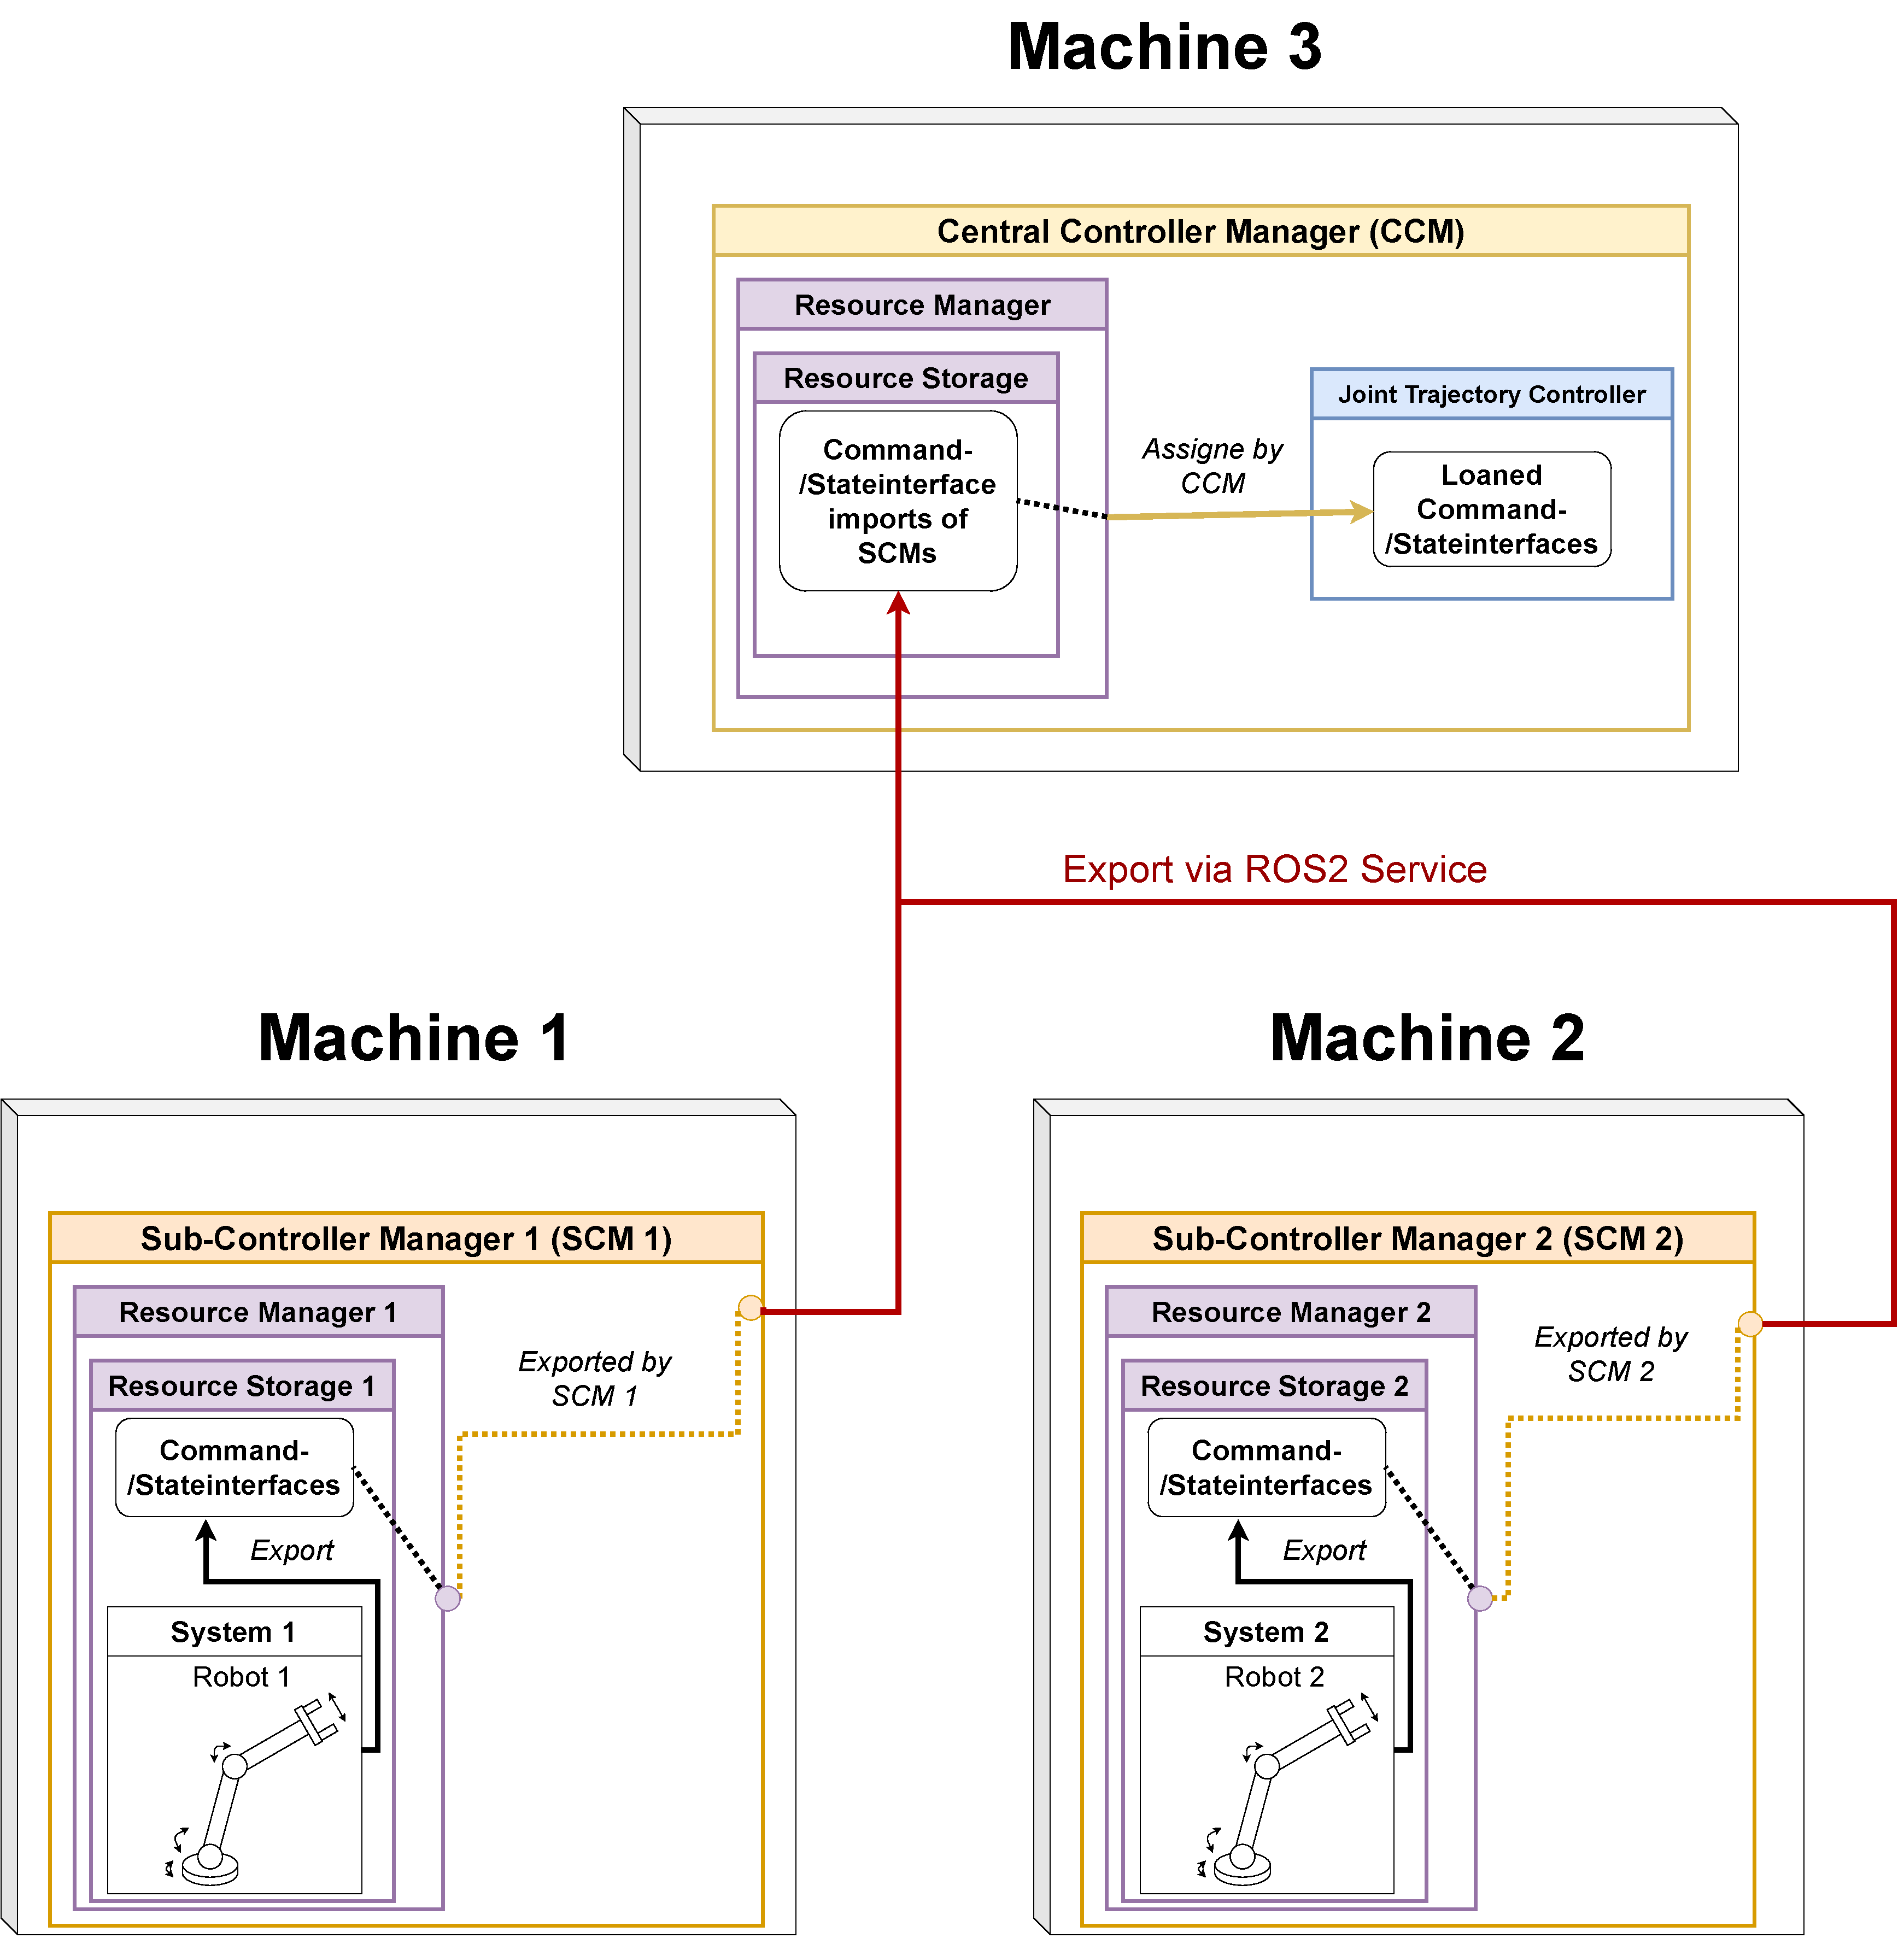
\includegraphics[width=1\textwidth]{Figures/c6/test_scenario_1.drawio.pdf}
	\caption{Schematic overview of the conceptual design of the system for the first test.}
	\label{c6_fig_test_scenario_1}
\end{figure}
\section{test 2}
\begin{figure}[htbp]
	\centering
	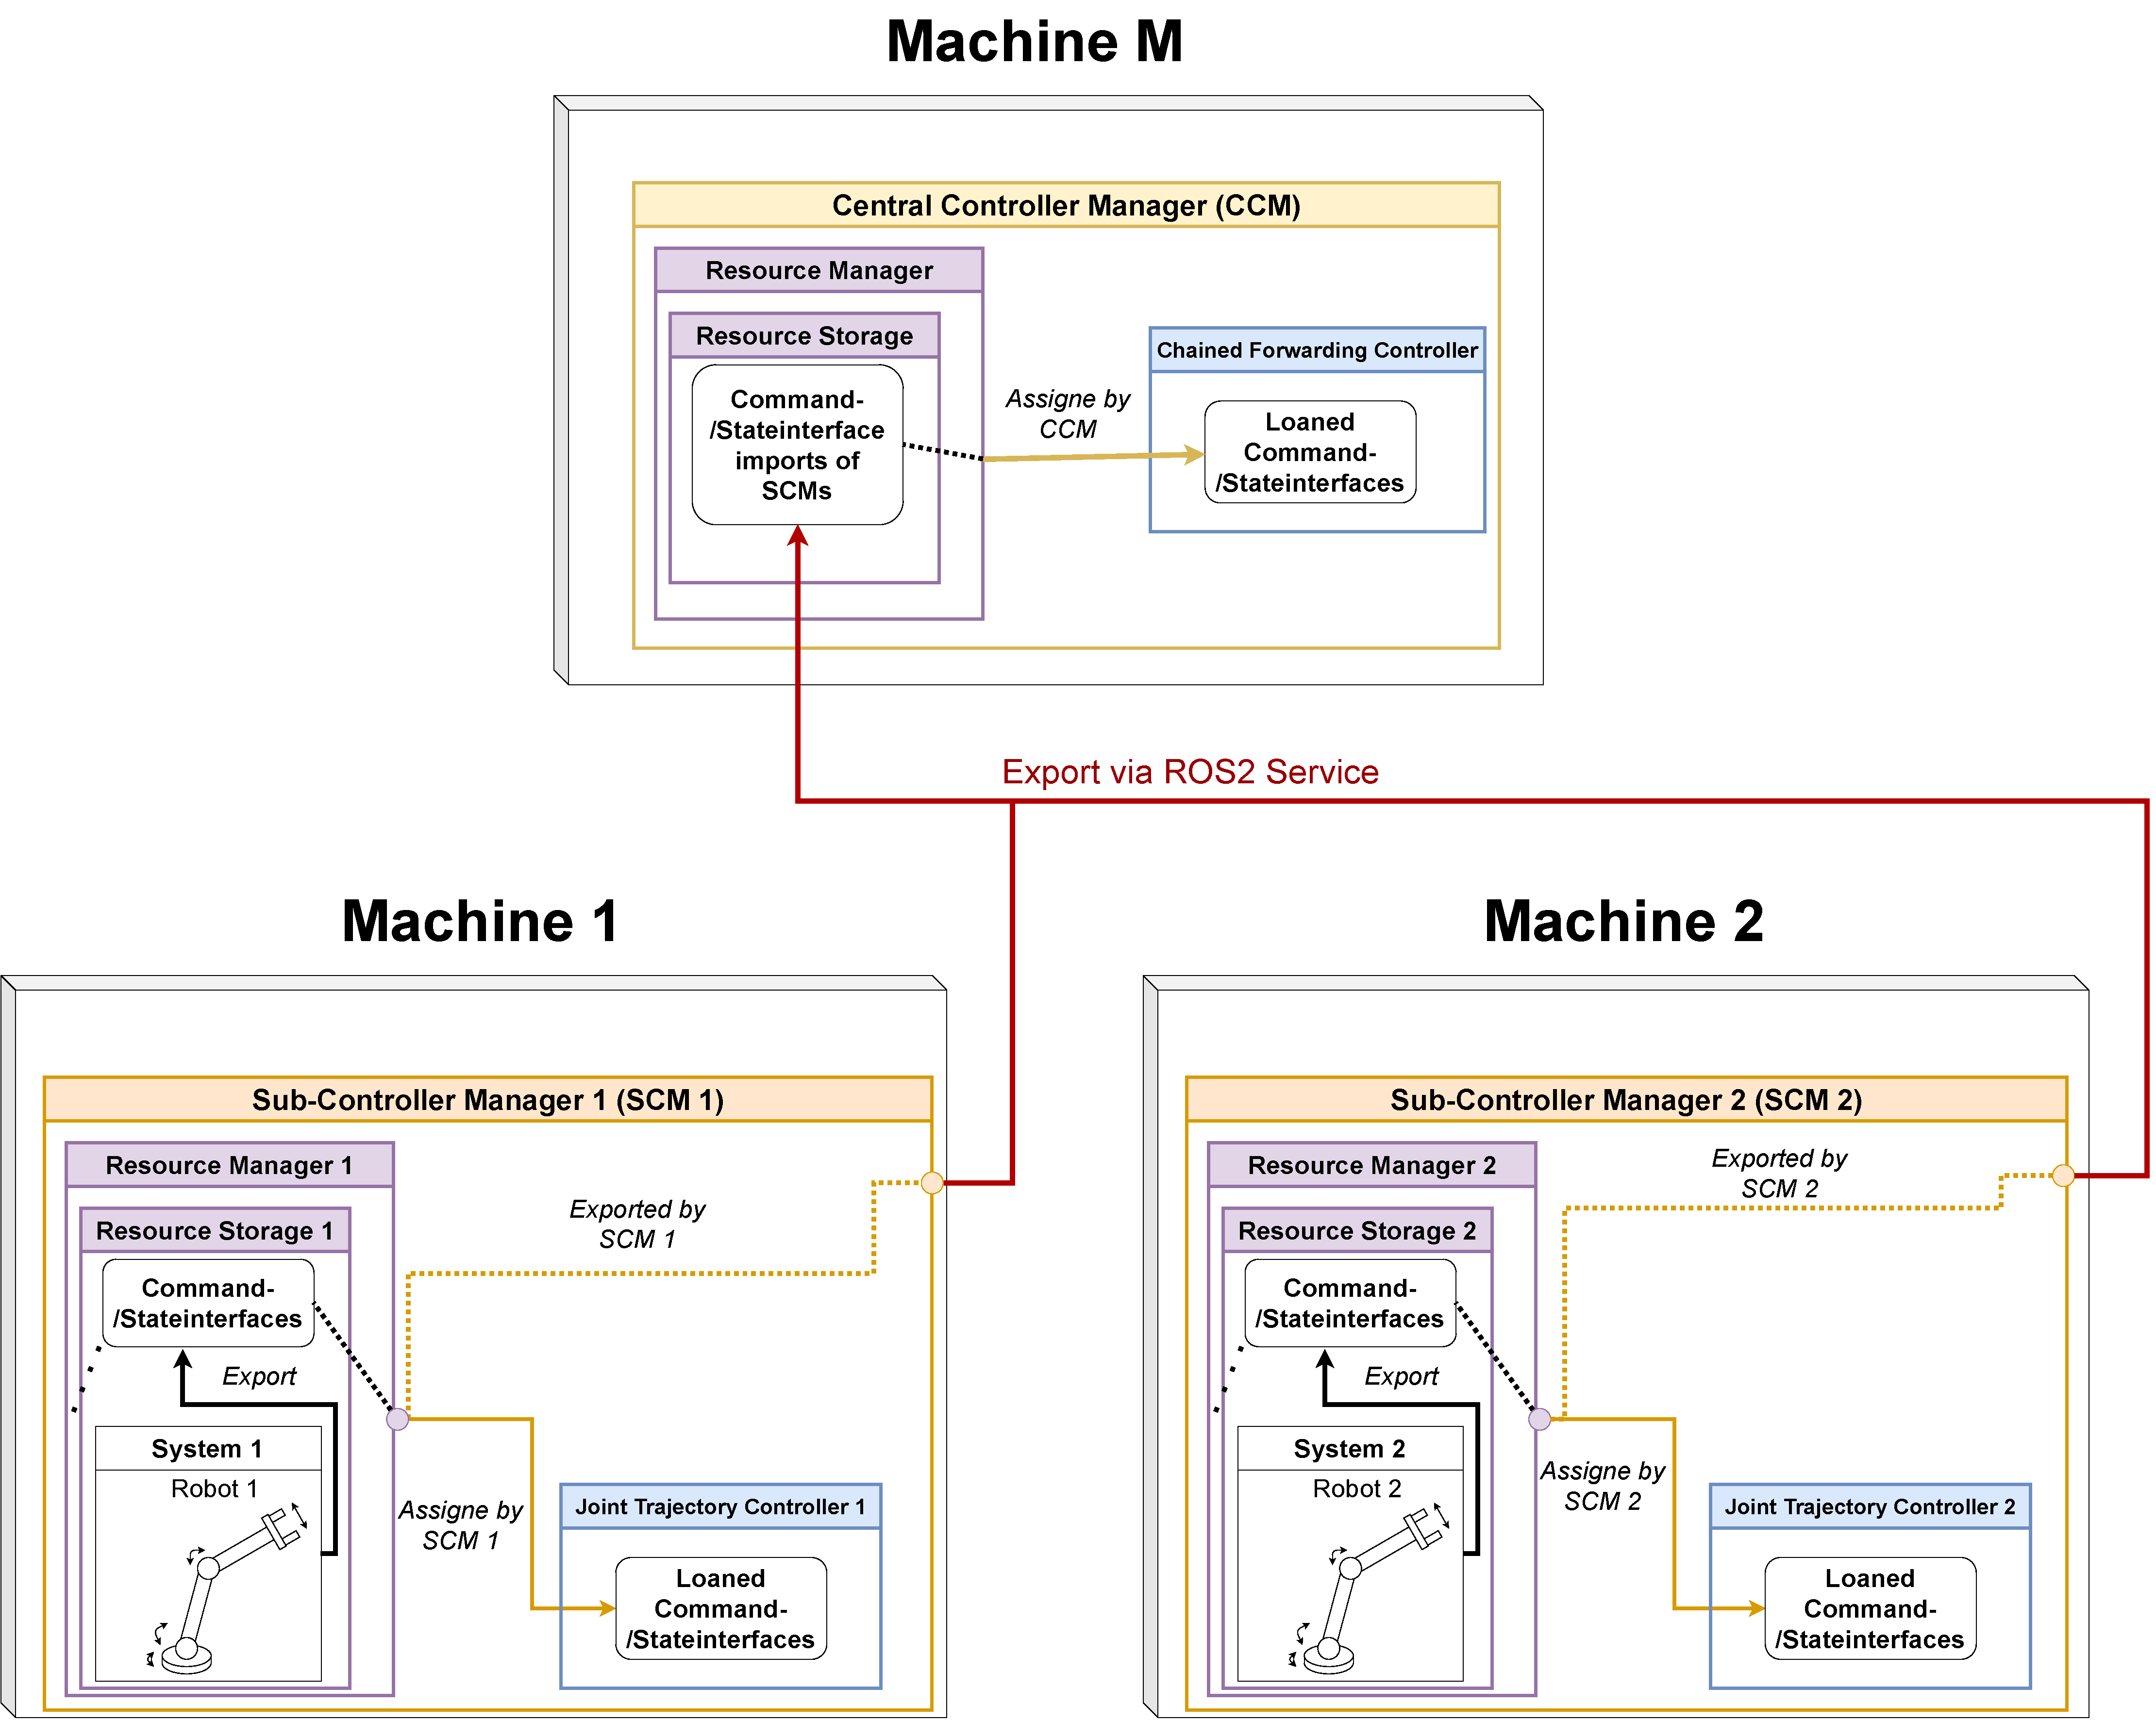
\includegraphics[width=1\textwidth]{Figures/c6/test_scenario_2.drawio.pdf}
	\caption{Schematic overview of the conceptual design of the system for the second test.}
	\label{c6_fig_test_scenario_2}
\end{figure}

\section*{Site Note}
Concept has also been tested on KUKA KR 16-2 KUKA KR 5 but because of how they are placed evaluation setup could not be conducted.
\missingfigure{Please add some figures}


% %% ==============================
% Part is used only in PhD thesis
\part{The Evaluation}
\chapter{\iflanguage{ngerman}{Diskussion}{Discussion}}
\label{sec:discussion}
%% ==============================




%% ==============================
\chapter{\iflanguage{ngerman}{Zusammensaffung und Ausblick}{Conclusion and Outlook}}
\label{sec:conclusion_and_outlook}
%% ==============================
In  this thesis, a concept for distributed control of multiple robots with the \gls{r2c} framework was proposed, implemented and evaluated. The main objective was to design an alternative concept to the shared-memory design of \gls{r2c}, that enables distributed control of robot systems with the framework. Further, the concept should allow for different distributed control architectures, while minimizing the impact of change on existing controllers and drivers. \newline
The proposed architecture consists of a central controller manager and multiple sub-controller managers. New distributed \glspl{si} and \glspl{ci} have been introduced, as well as wrapper classes for the old \glspl{si} and \glspl{ci}. The sub-controller managers can then export their \gls{si} and \gls{ci}, allowing the exchange of hardware states and commands over the network. This concept relies heavily on existing concepts from \gls{ros2} such as topics, publisher, subscribers and services.\newline
With the proposed concept, two different distributed control architectures can be realized, namely "distributed drivers" and "distributed chained control". In the "distributed drivers" case, the controller runs on one machine, while the drivers handling communication with the hardware run on separate machines. This allows for example to flexibly control multiple robots, where the robots are controller on one computer by a central controller and the communication is handled separately by the sub-controller managers on different machines. With the "distributed chained control" case, controllers can be distributed on multiple machines and then chained to each other. Meaning, the output of a controller running on the central controller manager can be chained to the input of a controller running in a sub-controller manager on a different machine. This allows for hierarchical control architectures, where a high level controller runs on the central controller manager, while low level controller and communication is handled in the sub-controller managers on different machines.\newline
The concept was evaluated using three different off the shelf laptops and two KUKA KR3 R540. The influence of the used \gls{rmw} and the choosen \gls{qos} on the performance was investigated. For the evaluation, the two robots were coupled with a distance sensor. Then trajectories were executed, where the distance between the two end effectors of the robot should stay the same if the robots move simultaneous. During the execution of the motion, the distance change has been plotted.\newline
In the first experiment, the "distributed drivers" case was investigated. A central controller manager with a \textit{JointTrajectoryController} was used. Additionally, two sub-controller managers, with each of them having the drivers for communication with the robots running, were used. The \glspl{rmw} Fast DDS, Cyclone DDS and Connext DDS were used. A reliable and a sensor profile were tested as well. The commands issued for the execution of the trajectories were all created by the central controller manager's \textit{JointTrajectoryController}. The measurements indicated that due to the implicit time synchronization, the robots move in a nearly synchronous manner. Small deviation in the micrometer range could be measured. The movement was repeatable and reliable. Further, the sensor profile always performed better than the reliable profile, regardless of the \gls{rmw}. The results for Fast DDS and Cyclone DDS are nearly similar. Both outperform Connext DDS. With both Fast DDS and Cyclone DDS no jitter of the robots could be observed. However, with Connext DDS as \gls{rmw} there was a permanent jitter during the execution present.\newline
In the second experiment, the "distributed chained control" case was investigated. In this experiment, each of the sub-controller managers had in addition to the drivers a \textit{JointTrajectoryController} running. The input of the \textit{JointTrajectoryControllers} were chained to the output of the central controller manager's \textit{ForwardCommandController}. The \textit{ForwardCommandController} did then send the same  "Trajectory message" via the \glspl{ri} to the \textit{JointTrajectoryControllers}. The measurements for this result do indicate that the concept works. No jitter could be measured. However, as the commands for the execution of the trajectory are calculated by each of the \textit{JointTrajectoryControllers} in the sub-controller managers individually, there is no time synchronization between the two. As a result, the execution is not started in complete synchronization and further mechanisms such as a synchronized time between the machines are necessary.

The presented work would benefit from exploring the impact of synchronized time across different computers by making use of for example the time precision protocol (PTP). In addition, Zenoh as \gls{rmw} could be investigated. As of the time of writing, there is no implementation of Zenoh as \gls{rmw} existed, but a bridge for \gls{dds} exists. This should in theory allow to route all the \gls{dds} traffic through Zenoh. This however did not work and could not be further investigated. Last, the longest continuous execution of the periodic motion was around 15 minutes. While the robots did repeat their motion consistent, measured at industrial standards, where robots need to run for days or even weeks this is not a very long time. Therefore, a longtime test could be conducted.
% \begin{itemize}
%     \item Other middlewares
%     \item over Wi-Fi (lossy ...)
%     \item Ordered package delivery
%     \item time synchronized network (was not feasible only one network card per laptop. no special hardware and gps clock.)
%     \item longtime run (max was about 15 min=)
% \end{itemize}

%% --------------------
%% |   Bibliography   |
%% --------------------
\Bibliography{\mybibliographyfiles}

%% ----------------
%% |   Appendix   |
%% ----------------
% \cleardoublepage
%% appendix.tex
%%

%% ==============================
\Appendix
\label{ch:Appendix}
%% ==============================
\section{Quality of Service Profiles}\label{sec:app-qos}
\subsection*{Sensor Profile}
\lstset{language=C++,basicstyle=\scriptsize}
\begin{lstlisting}[caption=The used sensor profile.,label=ca_code_sensor_profile]
static const rmw_qos_profile_t rmw_qos_profile_sensor_data = {
  RMW_QOS_POLICY_HISTORY_KEEP_LAST,
  5,
  RMW_QOS_POLICY_RELIABILITY_BEST_EFFORT,
  RMW_QOS_POLICY_DURABILITY_VOLATILE,
  RMW_QOS_DEADLINE_DEFAULT,
  RMW_QOS_LIFESPAN_DEFAULT,
  RMW_QOS_POLICY_LIVELINESS_SYSTEM_DEFAULT,
  RMW_QOS_LIVELINESS_LEASE_DURATION_DEFAULT,
  false};
\end{lstlisting}
\subsection*{Reliable Profile}
\begin{lstlisting}[caption=The used reliable profile.,label=ca_code_sensor_profile]
static const rmw_qos_profile_t rmw_qos_profile_reliable = {
  RMW_QOS_POLICY_HISTORY_KEEP_LAST,
  1,
  RMW_QOS_POLICY_RELIABILITY_RELIABLE,
  RMW_QOS_POLICY_DURABILITY_VOLATILE,
  RMW_QOS_DEADLINE_DEFAULT,
  RMW_QOS_LIFESPAN_DEFAULT,
  RMW_QOS_POLICY_LIVELINESS_SYSTEM_DEFAULT,
  RMW_QOS_LIVELINESS_LEASE_DURATION_DEFAULT,
  false};
\end{lstlisting}

% Remove if needed
%% -----------------------------
%% |   List of Figures/Tables  |
%% -----------------------------
\includeglossary
\includeacronyms
\inculdelistoffigures
\inculdelistoftables
\inculdelistoflistings
\inculdelistofalgoritms

%% --------------------
%% |   MyBib Entry    |
%% --------------------
\addmybibentry

%% --------------------------------
%% |   How to use this document   |
%% --------------------------------
%\includehowtouse

\end{document}
